\documentclass[12pt,a4paper]{article}

\usepackage[utf8]{inputenc}
\usepackage[T1]{fontenc}
\usepackage[margin=2.5cm]{geometry}
\usepackage{setspace}
\usepackage{natbib}
\usepackage{hyperref}
\usepackage{booktabs}
\usepackage{array}
\usepackage{amsmath}
% \usepackage{microtype}  % disabled: triggers font expansion error in this MiKTeX install
\usepackage{graphicx}
\usepackage{caption}
\usepackage{subcaption}
\usepackage{float}

\graphicspath{{../figures/}}
\doublespacing
\bibliographystyle{agsm}

\title{Institutional Secularism and Women's Welfare:\\
A Cross-National Panel Analysis, 2007--2022}
\author{MDM3 Project --- University of Bristol}
\date{}

\begin{document}

\maketitle

\begin{abstract}
\noindent We estimate the association between institutional secularism and women's welfare across 166 countries from 2013 to 2022. The focal predictor is a composite secularism index built as an equal-weighted average of z-scored components across two dimensions: an institutional dimension (three \emph{structural} Pew Global Restrictions on Religion sub-items measuring state religion, religious law, and religious courts) and a behavioural dimension (four World Values Survey religious-intensity items). Four further Pew items (apostasy laws, blasphemy laws, government religious favouritism) and V-Dem's religious-freedom index are excluded from the composite on circularity grounds --- each measures how the state treats people on religious grounds, which overlaps mechanically with the outcome --- and enter the analysis only as standalone sub-item focals in the decomposition regressions. The outcome is a composite women's treatment index built from the World Bank's Women, Business and the Law data combined with health and political-representation indicators. Four estimators are reported: cross-sectional OLS, two-way fixed-effects panel, a Mundlak correlated random-effects decomposition, and a system generalised method of moments estimator that we report for transparency but exclude from the headline conclusions. The composite cross-sectional coefficient in 2020 is $-0.097$ ($p = 0.017$), and the Mundlak between-country component is $-0.119$ ($p = 0.004$). The within-country panel signal, by contrast, is null or mildly wrong-signed ($+0.024$, $p = 0.09$ in TWFE; $+0.024$, $p = 0.07$ in the Mundlak within component). The between-country component is roughly five times the within-country component in magnitude and opposite in sign. A long-difference specification over 2013--2022 confirms the within-country null at the decade horizon ($\hat\beta = +0.053$, $p = 0.17$), ruling out short-run noise and WVS interpolation as the binding explanation. The significant cross-section is carried primarily by the WVS behavioural dimension: the institutional-only composite variant is not statistically distinguishable from zero in either cross-section year, whereas the full equal-weighted composite retains a significant negative coefficient. We read the evidence as a structural cross-national difference rather than a within-country mechanism over the 2013--2022 window; the 10-year panel is short for institutional secularism, and the within-country movement in the composite's behavioural dimension is substantially interpolated between WVS waves. Apostasy laws are retained as the strongest individual sub-item; they survive every robustness check with a cross-country coefficient of $-0.126$ ($p = 0.001$) and a within-country coefficient of $-0.018$ ($p = 0.07$, $p = 0.006$ under Driscoll--Kraay standard errors). Religious courts, the prior focal predictor in earlier versions of this analysis, are retained as a legacy null.
\end{abstract}

\section{Introduction}

Whether religion shapes women's welfare is a long-running question in comparative political economy. \citet{Ross2008}, \citet{Seguino2011} and \citet{HtunWeldon2015} establish that religion-and-gender comparisons typically conflate two distinct sources of variation: differences \emph{between} countries that institutionalise particular religious arrangements and changes \emph{within} countries that adopt or repeal those arrangements. A pooled regression coefficient mixes the two, and the policy-relevant interpretation differs sharply depending on which is dominant. If the relationship runs through within-country change, then institutional reform predicts welfare improvement. If it runs through structural between-country differences, then the relationship is a feature of country composition and tells us less about the consequences of reform.

This paper estimates the relationship between a composite index of institutional secularism and a composite measure of women's welfare across 166 countries from 2013 to 2022. The focal predictor is a construct-level summary: an equal-weighted average of z-scored components across two dimensions (three structural GRI legal-institution items and four WVS religious-intensity items). Building the focal predictor as a composite addresses a limitation of prior work on this dataset, which treated the individual Pew GRI sub-items as parallel univariate predictors even though several are near-binary and identified off a handful of within-country changers. The composite is restricted to ``state-of-being'' measures; items that measure how the state treats people on religious grounds (apostasy laws, blasphemy laws, government religious favouritism, and V-Dem's religious-freedom index) are excluded from the composite to avoid partial mechanical overlap with the outcome, which is itself a measure of how the state treats women. Those four items appear in the analysis only as standalone sub-item focals in the decomposition regressions. The outcome is a $[0, 1]$ composite built from the World Bank's Women, Business and the Law (WBL) legal-rights data combined with health and political-representation indicators.

The empirical contribution is a four-tier identification strategy that escalates the demand placed on the data. The first tier estimates the cross-sectional correlation in two snapshot years (2014 and 2020). The second tier exploits the full panel with country and year fixed effects. The third tier estimates a dynamic panel using system generalised method of moments, which we report for transparency but exclude from the headline conclusions because it marginally violates the \citet{Roodman2009} bounds check. The fourth tier applies the Mundlak correlated random-effects decomposition, which separates the within-country and between-country components in a single specification \citep{Mundlak1978, BellJones2015}. As a within-country robustness complement we also run a long-difference specification \citep{AcemogluJohnsonRobinsonYared2008, BesleyPersson2011} that collapses the panel to a single decade-change observation per country; it tests whether the within-country null at the annual scale persists at the medium-run horizon and sidesteps the WVS linear-interpolation concern we return to in the Discussion.

The headline result runs one direction at the between-country level and the opposite direction within country. Cross-sectionally, a country scoring one point higher on the composite (a move from most secular to most religious on the normalised scale) is associated with a women's treatment index that is $0.097$ points lower in 2020 ($p = 0.017$). The Mundlak between-country component is $-0.119$ ($p = 0.004$). The within-country panel coefficient over the 2013--2022 window is $+0.024$ ($p = 0.09$ in TWFE, $p = 0.07$ in the Mundlak within component), wrong-signed for the prior and small in absolute magnitude. The between-country component is roughly five times the within-country component and the two point in opposite directions. The long-difference robustness specification confirms the within-country null at the decade horizon ($+0.053$, $p = 0.17$). We read this as structural rather than within-country: countries with more secular institutions have better women's welfare, but countries do not show that association developing as they move on the composite over a decade.

Two qualifications sit in the Discussion. First, the panel is short. Institutional secularism moves slowly, and the 2013--2022 window is too narrow for large within-country movement on most of the composite's structural legal-institutional components. Second, the composite's behavioural dimension draws on WVS survey intensity items that are interpolated between survey waves. In the T2 sample, $134$ of $166$ countries are changers on the composite when we count any movement; restricting to rows where the underlying WVS is observed in the wave year rather than interpolated brings the real-movement changer count across the full panel down to $107$ of $198$. The within-country movement in the composite therefore leans partly on interpolator arithmetic, and within-country evidence has to be read with that in mind.

The paper reports the individual Pew GRI sub-items as sub-item robustness entries. Apostasy is the strongest individual sub-item and survives every check in the battery: its cross-section coefficient in 2020 is $-0.119$ ($p = 0.003$), its Mundlak between-country coefficient is $-0.126$ ($p = 0.001$), and its within-country coefficient is $-0.018$ ($p = 0.07$ under entity-clustered SEs, $p = 0.006$ under Driscoll--Kraay). Religious courts is the prior focal predictor in earlier versions of this analysis; it is retained as a legacy null. Its coefficient is small and insignificant at every tier, and the variable is effectively binary in 2020 with $29\%$ within-country variance share and only 36 of 166 panel countries recording any movement, so the null is power-limited and partly a feature of the measurement.

The remainder of the paper proceeds as follows. Section 2 describes the data and the construction of the composite secularism index. Section 3 sets out the four-tier empirical strategy. Section 4 reports the headline coefficients with the supporting figures. Section 5 presents the robustness battery, including the long-difference specification. Section 6 discusses the substantive interpretation of the structural between-country result and the within-country null. Section 7 lists limitations. Section 8 concludes. Appendix A presents supporting robustness checks for the individual GRI sub-items and lists the checks we computed but excluded from the body, with reasons.

\section{Data}

\subsection{Outcome: Women's Treatment Index}

The dependent variable is a composite women's treatment index constructed from the World Bank's Women, Business and the Law (WBL) dataset, the World Bank's World Development Indicators (health and labour-force outcomes), and political-representation data (women in parliament and ministerial positions). The composite is built by the script \texttt{scoring.py} in two layers. The de-jure layer averages eight WBL legal-rights groups (Mobility, Workplace, Pay, Marriage, Parenthood, Entrepreneurship, Assets, Pension; the WBL labels in the underlying data are slightly different). The de-facto layer averages two outcome groups (Health and Political Representation). The overall score is the equal-weighted average of the two layer scores, on a $[0, 1]$ scale where higher means better. The two-layer construction prevents the outcome from being dominated by either the legal-rights count or the outcome metrics individually.

Variables on different scales are normalised before averaging. Continuous variables that have natural bounds (life expectancy, with UNDP HDI bounds of 20 and 85) use those fixed bounds. The remaining continuous variables are min-max normalised on the data, with a 1st--99th percentile winsorisation step that prevents single-country outliers from compressing the rest of the distribution. Two negatively-coded variables (adolescent fertility and maternal mortality) are inverted so that higher values mean better outcomes everywhere.

A composite index requires a non-missingness threshold to avoid noisy partial scores. Country-years with fewer than eight of the thirteen underlying outcome variables observed are dropped. After this filter the cleaned outcome file covers 187 countries and 2{,}057 country-year observations from 2013 to 2023. The relevant column in \texttt{data/outcome\_wbl.csv} is \texttt{wbl\_treatment\_index}. The estimation panel is then defined by the merge with the predictor file (described in Section 2.4), which restricts the analysis to 2013--2022.

\subsection{Focal Predictor: Composite Secularism Index}

The focal predictor, \texttt{composite\_secularism\_norm}, is an equal-weighted z-score composite built across two dimensions, all oriented so that higher values indicate a more religious society. The construction is implemented by \texttt{analysis.utils.build\_secularism\_composite} and applied at load time inside the analysis pipeline; the composite is not stored on disk. An earlier version of this composite aggregated eleven inputs across three dimensions and included four further items (apostasy laws, blasphemy laws, government religious favouritism, and the V-Dem religious-freedom index); those items were removed from the composite in a 2026-04-16 rebuild on circularity grounds and now enter the analysis only as standalone sub-item focals in the decomposition regressions. The rationale is stated explicitly in the next paragraph.

The institutional dimension aggregates three \emph{structural} Pew Global Restrictions on Religion sub-items: whether a state religion exists (\texttt{gri\_state\_religion\_norm}), the role of religious law in the legal system (\texttt{gri\_religious\_law\_norm}), and the formal role of religious courts (\texttt{gri\_religious\_courts\_norm}). Each of these captures a constitutional fact about how religion is embedded in state institutions, without itself being a policy that acts on individuals. The behavioural dimension uses four World Values Survey religious-intensity items that capture population-level attitudes rather than state policy: self-reported importance of religion (\texttt{wvs\_imprel\_norm}), importance of God (\texttt{wvs\_godimp\_norm}), belief in God (\texttt{wvs\_godbel\_norm}), and confidence in religious institutions (\texttt{wvs\_confch\_norm}).

Each input column is z-scored across the sample (NaN-aware). Z-scores are averaged within each of the two dimensions, and the two dimension z-scores are then row-averaged. If one dimension is entirely missing for a row, the row's composite equals the observed dimension (a dimension-fallback rule), which keeps most rows usable in the presence of patchy WVS coverage. The resulting series is passed through a robust min-max normalisation with 1st--99th percentile winsorisation so that the composite is on a $[0, 1]$ scale that matches the rest of the predictor set. Sign alignment is verified by asserting that the composite is positively correlated with the fully-covered institutional item \texttt{gri\_state\_religion\_norm}; the assertion passes without modification.

\paragraph{Why four inputs were removed.} The earlier eleven-input composite mixed two conceptually distinct things: measures of how religious a society is (state religion, religious law, religious courts, and the WVS attitudinal items), and measures of how the state treats people on religious grounds (\texttt{gri\_apostasy\_norm}, which codes whether the state criminalises leaving a religion; \texttt{gri\_blasphemy\_norm}, whether it criminalises blasphemy; \texttt{gri\_gov\_favour\_norm}, whether one religion is officially favoured in policy; and \texttt{v2clrelig\_norm}, V-Dem's religious-freedom index). The outcome \texttt{wbl\_treatment\_index} measures how the state treats women on legal grounds. Penal codes, family law, and constraints on individual religious freedom are generated by the same legal-institutional machinery that sets women's legal rights, so including treatment-of-people-on-religious-grounds variables inside the composite created a partial mechanical overlap with the outcome and inflated the cross-sectional coefficient beyond what ``religiosity as a state of being'' explains. The rebuild replaces the composite with the seven inputs listed above, which are all state-of-being measures; the four removed items remain in the analysis as standalone sub-item focals in the T1, T2, and T4 decomposition regressions, where the cleaner \texttt{GRI\_PANEL\_COLS} spec keeps them visible without conflating them with the composite headline. The full rebuild audit is in \texttt{reviews/2026-04-16\_secularism-composite-rebuild.md}. An important consequence is that the composite's significant cross-section is now driven primarily by the behavioural (WVS) dimension; the institutional-only variant (three structural GRI items alone) is not significant in 2014, while the behavioural-only variant carries a coefficient of about $-0.13$. We surface this decomposition honestly in the weight-sensitivity results below and in the within-country discussion in \S\ref{sec:within-null} rather than treating the composite as a unitary structural construct.

We report the composite under two alternative dimension weightings as a sensitivity check on the equal-weight choice. \texttt{composite\_secularism\_instonly\_norm} drops the behavioural dimension entirely and takes the z-score mean of the three structural institutional GRI items alone. \texttt{composite\_secularism\_covwt\_norm} weights each of the two dimensions by its panel-wide non-null row fraction, where the WVS behavioural dimension's coverage is computed on pre-interpolation wave years so the variant is informative even when the main composite is built on post-interpolation data. The covwt composite is still constructed from the post-interpolation WVS values; only the weight the behavioural dimension receives is reduced to reflect its real-coverage share. Readers should treat covwt as a blended composite with a small interpolator-exposed behavioural share, not as a WVS-real-only variant. The raw dimension coverages on the merged panel are high for institutional (all three structural GRI columns observed) and low for behavioural (all four WVS columns observed in a real wave year), so the coverage-weighted composite places most of its weight on the institutional dimension against the equal-weight share of $50\%$ on each. Table \ref{tab:weight-sensitivity} reports the headline coefficients under the three weightings; values are regenerated from \texttt{results/results.csv} after the 2-dimension rebuild.

\begin{table}[h!]
\centering
\caption{Composite secularism coefficients under three dimension weightings. Institutional-only drops the behavioural dimension and averages the three structural institutional GRI items. Coverage-weighted downweights the behavioural dimension by its pre-interpolation panel coverage. All rows use the same estimation samples as the main composite.}
\label{tab:weight-sensitivity}
\begin{tabular}{lccc}
\toprule
Specification & Equal & Institutional-only & Coverage-weighted \\
\midrule
T1 2020 with GDP ($\hat\beta$, $p$)      & $-0.097$, $0.017$   & $-0.061$, $0.12$    & $-0.062$, $0.10$   \\
T2 with GDP within ($\hat\beta$, $p$)    & $+0.024$, $0.09$    & $+0.004$, $0.70$    & $+0.007$, $0.48$   \\
T4 Mundlak within ($\hat\beta$, $p$)     & $+0.024$, $0.07$    & $+0.004$, $0.69$    & $+0.007$, $0.46$   \\
T4 Mundlak between ($\hat\beta$, $p$)    & $-0.119$, $0.004$   & $-0.055$, $0.17$    & $-0.059$, $0.12$   \\
\bottomrule
\end{tabular}
\end{table}

Under the 2-dimension composite, the three weightings produce a clean gradation on the structural--behavioural axis. Institutional-only averages the three structural GRI items alone (state religion, religious law, religious courts) and is a pure near-categorical composite with no behavioural input; coverage-weighting puts most weight on the institutional dimension because the WVS behavioural dimension has low real-wave coverage; equal-weight splits weight $50/50$. The cross-sectional and between-country coefficients retain their negative sign under every weighting but attenuate as weight moves away from the behavioural WVS dimension: the institutional-only variant is the smallest in magnitude and not statistically distinguishable from zero in the cross-section, while the equal-weight composite retains a significant negative coefficient on account of the behavioural share. The within-country coefficient is small, wrong-signed, and not reliably distinguishable from zero across all three weightings. The three-way comparison settles a specific claim: the significant cross-section effect of the composite is carried by the WVS behavioural dimension, not by the structural GRI dimension alone. This is the same direction as the no-interpolation variant reported in \S\ref{sec:within-null}, and readers should treat the composite as a blended construct whose headline coefficient reflects population-level religious attitudes more than it reflects the constitutional architecture of state--religion relations.

We also build and report \texttt{composite\_secularism\_pca\_norm} as a robustness variant. The PCA variant standardises the seven inputs and takes the first principal component; the loading on \texttt{gri\_state\_religion\_norm} is used to fix the sign. Three imputation strategies are compared in \texttt{results/pca\_loadings\_comparison.csv}: column-mean imputation, listwise deletion on complete cases, and iterative EM imputation via scikit-learn's \texttt{IterativeImputer}. EM imputation is adopted as the primary PCA variant because it preserves the full merged panel while avoiding the variance shrinkage that mean imputation introduces on the low-coverage WVS rows. The three imputations recover essentially the same first-component loadings, so the choice does not change the latent factor the PCA recovers; it changes the sample on which it is fit and the proportion of within-sample variance the first PC can absorb. The first principal component loads most heavily on the four WVS behavioural items and less on the three structural GRI institutional items, which mirrors the equal-weight composite's implicit weighting once z-scoring is taken into account. The PCA variant is therefore a cross-check on the equal-weight composite rather than an independent construction. Cross-sectionally the two composites agree closely in sign and magnitude; within-country they also both produce the small wrong-signed positive estimate that the equal-weight composite carries, with the exact magnitudes reported in \texttt{results/results.csv}.

One diagnostic caveat for the composite matters for interpretation. The composite is continuous by construction, so in a panel sample a large majority of countries move on it in every year. The ``number of changer countries'' diagnostic that was informative for the near-binary sub-item predictors is less useful for the composite: $134$ of $166$ countries in the T2 sample are changers, a majority but not the saturation the prior eleven-input composite produced. The more useful within-country variation diagnostic for the composite is its within-country standard deviation, which is $0.062$ on the $[0, 1]$ scale, a little larger than the $0.039$ that the earlier eleven-input composite recorded because removing the slow-moving V-Dem religious-freedom input raises the remaining composite's year-on-year movement. To separate real within-country movement from WVS-interpolation arithmetic, we additionally report a changer count restricted to rows where the underlying WVS wave was actually observed rather than linearly interpolated: on that restriction, $107$ of $198$ countries are changers. Within-country inference for the composite must acknowledge that some of its within-country movement is interpolator-driven.

The WVS series is linearly interpolated within country between survey waves, with $\pm 2$-year edge fill. The interpolation is flagged in \texttt{wvs\_interpolated} and is documented in \texttt{docs/methods\_log.md}. Only $107$ of the $198$ panel countries have any real wave-on-wave WVS movement at all across the 2007--2022 window; the remaining $91$ countries' WVS contribution to the main composite is pure linear interpolation between at most one observed wave. To quantify how much of the composite's within-country signal depends on the interpolator, we also build \texttt{composite\_secularism\_real\_norm}: an equal-weighted composite constructed with the four WVS columns masked to missing on every row where \texttt{wvs\_interpolated} equals one. The behavioural dimension of the real variant therefore contributes only real wave-year observations. It is reported as a robustness row in the headline tier specifications; where the main composite's within-country coefficient is driven by interpolator movement rather than by real wave-observed attitudinal change, the real variant's coefficient will move.

\subsection{Controls}

Three V-Dem governance indices enter as controls: \texttt{v2x\_rule\_norm} (rule of law), \texttt{v2x\_civlib\_norm} (civil liberties), and \texttt{v2x\_egal\_norm} (egalitarian component), all from the V-Dem v13 dataset.\footnote{V-Dem Institute, University of Gothenburg, \url{https://www.v-dem.net}.} These absorb the broad institutional environment within which religious institutions operate. Specifications labelled ``with GDP'' add a fourth control, \texttt{log\_gdppc\_norm}: log GDP per capita in constant 2015 USD, robust min-max normalised to $[0, 1]$. The normalisation is important for interpretation: coefficients on \texttt{log\_gdppc\_norm} are per unit of the normalised scale, not per log-point of GDP.

\subsection{Sample}

The estimation sample varies by specification. The cross-sectional models in 2014 and 2020 include 170 countries (164--166 after the GDP control is added, due to GDP missingness for some small economies). The two-way fixed-effects panel covers 166 countries across 10 years (2013--2022) for $1{,}648$ country-year observations in the with-GDP specification, and 170 countries for $1{,}700$ observations in the no-GDP specification. The system-GMM panel uses $1{,}316$ observations after lag construction. The full inventory of normalisation, interpolation and missing-data choices is documented in \texttt{docs/methods\_log.md}.

\section{Empirical Strategy: Tiered Identification}

The four estimators are not parallel alternatives. They form an escalating identification strategy: each tier addresses a threat to validity that its predecessor cannot. Throughout, $W_{it}$ denotes the women's treatment index for country $i$ in year $t$, $S_{it}$ the composite secularism predictor, $\mathbf{X}_{it}$ the V-Dem governance controls and (where included) log GDP per capita, $\alpha_i$ time-invariant country effects, $\lambda_t$ year effects, and $\varepsilon_{it}$ an idiosyncratic error.

\subsection{Tier 1: Cross-Sectional OLS}

\subsubsection{Specification}

Tier 1 estimates the cross-sectional relationship at two snapshot years, 2014 and 2020:
\begin{equation}
W_i = \alpha + \beta S_i + \boldsymbol{\gamma}^{\prime} \mathbf{X}_i + \varepsilon_i.
\end{equation}
Standard errors use the HC3 heteroskedasticity-consistent estimator, a jackknife-style refinement of the standard White correction that retains correct rejection rates at the sample sizes here ($N \approx 170$) where the simpler HC0 and HC1 estimators over-reject. \citet{CameronMiller2015} provides a current treatment.

\subsubsection{Motivation}

Cross-sectional OLS is the transparent benchmark. It establishes the bivariate and conditional correlations on the maximum sample, is straightforward to reproduce, and lets us compare the estimated coefficients directly with prior work that has used cross-section regressions on similar outcomes \citep{Ross2008, Seguino2011, HtunWeldon2015}. The two snapshot years (2014 and 2020) are chosen because they bracket a decade of variation and because data coverage is complete in both years.

\subsubsection{Literature Precedent}

Cross-sectional OLS is the dominant first-tier estimator in cross-national religion-and-gender research. \citet{Ross2008} uses time-averaged cross-section OLS as the primary estimator in his oil-Islam-women study, with panel fixed effects only as a robustness check; the design treats the cross-section as the interpretively central result. \citet{Seguino2011} estimates seven gender-equality outcomes against religiosity and denomination shares across roughly 64 countries, again with OLS as the headline estimator and 2SLS/3SLS as validation. \citet{HtunWeldon2015} uses cross-national regression in a 70-country study to estimate whether state endorsement of religious authority predicts women's family-law rights. The pattern is consistent across this literature: the cross-section anchors the bivariate and conditional correlations, which subsequent panel work then validates.

\subsection{Tier 2: Two-Way Fixed-Effects Panel}

\subsubsection{Specification}

Tier 2 pools all country-year observations from 2013 to 2022 and estimates
\begin{equation}
W_{it} = \beta S_{it} + \boldsymbol{\gamma}^{\prime} \mathbf{X}_{it} + \alpha_i + \lambda_t + \varepsilon_{it}.
\end{equation}
Country fixed effects $\alpha_i$ absorb every time-invariant country characteristic (history, culture, geography, colonial inheritance, baseline legal tradition) that might be correlated with both the composite predictor and the outcome. Year fixed effects $\lambda_t$ absorb common global shocks (financial crisis, pandemic, global feminist mobilisation). Standard errors are clustered at the country level. The estimator is implemented with \texttt{linearmodels.PanelOLS(entity\_effects=True, time\_effects=True, cov\_type=``clustered'', cluster\_entity=True)}.

\subsubsection{Motivation}

If the unobserved country effects $\alpha_i$ are correlated with the secularism regressor, as is theoretically expected (the same colonial and cultural histories shape both religious institutional structure and women's legal rights), random-effects estimates are inconsistent and the within-estimator is appropriate \citep{Hausman1978}. Two-way FE projects the data onto its within-country, within-year residual variation, eliminating both time-invariant country confounders and period-specific global shocks \citep{AngristPischke2009}. Country-clustered standard errors handle the within-country serial correlation that conventional panel SEs underestimate \citep{BertrandDufloMullainathan2004}; \citet{CameronMiller2015} discusses cluster-robust inference in the unbalanced panel setting that applies here.

\subsubsection{Literature Precedent}

\citet{Seguino2011} applies country and survey-wave fixed effects in all panel specifications. \citet{BenNunBloom2016} uses time-series cross-sectional regression with country and year controls on 153 nations to predict women's rights from religious regulation indicators that are structurally similar to the inputs of our composite. \citet{HtunWeldon2015} extends the framework to family-law outcomes in a 70-country panel with religious power as the primary predictor. These studies establish two-way FE as both empirically prevalent and theoretically motivated for the present research question.

\subsection{Tier 3: System-GMM}

\subsubsection{Specification}

Tier 3 estimates a dynamic panel using the system generalised method of moments estimator \citep{BlundellBond1998}:
\begin{equation}
W_{it} = \rho W_{i,t-1} + \beta S_{it} + \boldsymbol{\gamma}^{\prime} \mathbf{X}_{it} + \alpha_i + \lambda_t + \varepsilon_{it}.
\end{equation}
The lagged outcome $W_{i,t-1}$ and the religious institutional regressors are treated as predetermined or endogenous, instrumented with lags of the endogenous variables in the differenced equation and lag-1 differences in the levels equation. Instrument matrices are collapsed to limit instrument proliferation, since the instrument count should not exceed the number of cross-sections \citep{Roodman2009}. Two-step GMM is used with finite-sample standard-error corrections. Instrument validity is assessed via the Hansen $J$-statistic and the Arellano--Bond AR(2) test on the differenced residuals.

\subsubsection{Motivation}

Two identification threats remain after Tier 2. First, the WBL-based welfare composite is highly persistent: scores in year $t$ are strongly predicted by scores in year $t-1$, because legal systems and welfare institutions change slowly. Failing to include a lagged dependent variable misspecifies the conditional mean. Including one in a TWFE model induces the \citet{Nickell1981} bias, which biases coefficients toward zero and is non-negligible at the dataset's $T = 10$ relative to $N \approx 166$. Second, the religious institutional predictors and the V-Dem governance controls are institutionally co-determined with women's welfare: countries with improving women's welfare may progressively constrain the jurisdiction of religious institutions; governance quality and women's rights co-evolve through shared political-economy channels. System-GMM addresses both: the lagged-DV instrumentation eliminates Nickell bias, and internal lagged instruments handle simultaneity without external instruments.

\subsubsection{Literature Precedent}

\citet{Achuo2024} is the closest published analogue: 142 countries from 1996 to 2020, the WBL Index as the outcome, institutional quality (rule of law, government effectiveness, regulatory quality) as the predictors, with System-GMM as a robustness estimator alongside Driscoll--Kraay standard errors and full Hansen and AR diagnostics. The match in sample frame, outcome variable and estimator design makes Achuo et al.\ the natural template for this tier.

\subsubsection{Diagnostic Caveat}

The System-GMM estimator in this application narrowly violates the Roodman bounds check. The autoregressive coefficient on $W_{i,t-1}$ from GMM marginally exceeds the pooled-OLS upper bound and sits well above the within-estimator lower bound. In a correctly-specified dynamic panel, the GMM estimate of $\rho$ should lie between these two bounds \citep{Roodman2009}; landing above the OLS upper bound suggests the moment conditions do not hold tightly in this dataset. The Hansen $J$-statistic does not reject instrument validity and the Arellano--Bond AR(2) test passes, so the standard endogeneity-test machinery is not raising further alarms, but the bounds violation is the binding concern. The T3 results are reported for transparency in Table~\ref{tab:headline} but are excluded from substantive interpretation. The dataset's $T = 10$ falls at the boundary of the small-$T$ large-$N$ regime where System-GMM is well behaved, which is a plausible explanation for the marginal violation. The T1, T2 and T4 estimates carry the headline conclusions.

\subsection{Tier 4: Mundlak Correlated Random Effects}

\subsubsection{Specification}

Tier 4 applies the \citet{Mundlak1978} correlated random-effects decomposition:
\begin{equation}
W_{it} = \beta_1 S_{it} + \beta_2 \bar{S}_i + \boldsymbol{\gamma}^{\prime} \mathbf{X}_{it} + \lambda_t + u_i + \varepsilon_{it},
\end{equation}
where $\bar{S}_i = T^{-1} \sum_t S_{it}$ is the country-level time average of the composite, $\lambda_t$ are year fixed effects, $u_i$ is a country-level random effect, and $\varepsilon_{it}$ is the idiosyncratic error. The model is estimated by GLS random effects with entity-clustered standard errors. The within-country coefficient $\beta_1$ measures how a change in the composite within a country relates to a change in the outcome. The between-country coefficient $\beta_2$ measures whether countries that on average score high on the composite also on average score high on the outcome.

\subsubsection{Motivation}

The TWFE estimator (Tier 2) identifies coefficients only from within-country temporal variation, discarding all between-country information by construction. The Mundlak approach retains both dimensions of variation in a single specification and provides a built-in diagnostic. If the between coefficient differs sharply in magnitude or sign from the within coefficient, the structural cross-national relationship dominates the within-country signal. The within coefficient $\beta_1$ is numerically equivalent to the TWFE coefficient from Tier 2, providing a consistency check (in this dataset, the difference is below $0.0003$ for the composite). \citet{BellJones2015} provides the modern treatment recommending the within-between decomposition over choosing between fixed and random effects in applied comparative work. For the present analysis the Mundlak decomposition is the interpretive headline: it is the cleanest single specification that separates the structural between-country gap from the within-country temporal signal.

\subsubsection{Long-Difference Robustness Complement}

The T2 and T4 within-country coefficients are identified off annual movement. In a short panel with slow-moving institutional regressors much of that annual movement is short-term noise, and the behavioural dimension of the composite is linearly interpolated between WVS waves so its annual variation is partly interpolator arithmetic. As a robustness complement we therefore also estimate a long-difference specification that collapses the panel to a single decade-change observation per country: $\Delta W_i = \alpha + \beta\,\Delta S_i + \boldsymbol{\gamma}^{\prime}\,\Delta\mathbf{X}_i + u_i$ with HC3 standard errors, $\Delta$ taken between the 2013 and 2022 endpoints. Long-differencing is the canonical fallback in comparative-development empirics when short annual panels cannot identify slow-moving institutional change \citep{AcemogluJohnsonRobinsonYared2008, BesleyPersson2011}; it throws away annual variation and any interpolator contamination between WVS waves. Results are reported in \S\ref{sec:longdiff} and inform the within-country reading in \S\ref{sec:within-null}, but the specification does not carry a separate headline tier.

\section{Results}

\subsection{Headline Coefficients}

Table~\ref{tab:headline} reports the coefficient on the composite secularism predictor across the four tiers plus a long-difference robustness row, with the equal-weight and PCA variants side by side. Apostasy and religious courts are reported as sub-item robustness entries. All coefficients are on the $[0, 1]$ welfare scale, so a coefficient of $-0.097$ corresponds to a $0.097$-point drop in the women's treatment index for a one-point increase in the (also $[0, 1]$-scaled) composite predictor.

\begin{table}[H]
\centering
\caption{Headline coefficients across the four tiers plus a long-difference robustness row. T1 reports the with-GDP cross-section in 2020. T2 reports the with-GDP TWFE panel ($n = 1{,}648$). T4 reports the within and between components from the Mundlak correlated random-effects model ($n = 1{,}648$). The long-difference row reports $\hat\beta$ on $\Delta$focal between 2013 and 2022 with GDP ($n = 163$, one observation per country, HC3 standard errors). Standard errors in parentheses. T3 system-GMM ($n = 1{,}316$) is reported in the main text but not in this table because it violates the Roodman bounds check. The composite (equal-weight) is the headline focal predictor; the composite (PCA) is a robustness variant. Apostasy is retained as the strongest individual sub-item robustness; religious courts is the legacy null predictor from earlier versions of this analysis. Source: \texttt{results/headline\_table.csv}.}
\label{tab:headline}
\begin{tabular}{lcccc}
\toprule
Tier & Composite (eq-wt) & Composite (PCA) & Apostasy & Courts \\
\midrule
T1 (2020 cross-section) & $-0.097$ ($0.041$)\textsuperscript{**} & $-0.116$ ($0.039$)\textsuperscript{***} & $-0.119$ ($0.040$)\textsuperscript{***} & $+0.017$ ($0.020$) \\
T2 (panel FE, with GDP) & $+0.024$ ($0.014$)\textsuperscript{$\dagger$} & $+0.022$ ($0.017$) & $-0.018$ ($0.010$)\textsuperscript{$\dagger$} & $-0.007$ ($0.007$) \\
T2 (Driscoll--Kraay SE) & $+0.024$ ($0.011$)\textsuperscript{**} & $+0.022$ ($0.012$)\textsuperscript{$\dagger$} & $-0.018$ ($0.007$)\textsuperscript{***} & $-0.007$ ($0.003$)\textsuperscript{**} \\
T4 within (Mundlak) & $+0.024$ ($0.013$)\textsuperscript{$\dagger$} & $+0.022$ ($0.016$) & $-0.018$ ($0.009$)\textsuperscript{$\dagger$} & $-0.007$ ($0.007$) \\
T4 between (Mundlak) & $-0.119$ ($0.042$)\textsuperscript{***} & $-0.151$ ($0.040$)\textsuperscript{***} & $-0.126$ ($0.038$)\textsuperscript{***} & $+0.042$ ($0.023$)\textsuperscript{$\dagger$} \\
\midrule
Long-difference (2013--2022) & $+0.053$ ($0.039$) & $+0.057$ ($0.038$) & -- & $-0.010$ ($0.013$) \\
\bottomrule
\end{tabular}
\smallskip
\\
{\footnotesize \textsuperscript{$\dagger$} $p < 0.10$, \textsuperscript{**} $p < 0.05$, \textsuperscript{***} $p < 0.01$. Long-difference row: HC3 standard errors, $n = 163$ countries; apostasy (--) is identified off nine changer countries only and is omitted here, see Appendix~\ref{sec:ld-details}. Courts long-difference is identified off 19 changer countries, below the power threshold for reliable inference.}
\end{table}

Five patterns stand out. First, the composite is negatively associated with women's welfare in the cross-section: the 2020 coefficient is $-0.097$ ($p = 0.017$), and the 2014 value is similar at $-0.100$ ($p = 0.005$). Second, the composite's Mundlak between-country coefficient is $-0.119$ ($p = 0.004$), confirming that the structural cross-national gap between more and less secular countries is negative and significant. Third, the composite's within-country coefficient over the 2013--2022 window is mildly positive rather than negative: $+0.024$ in both the TWFE and Mundlak within components, with $p \approx 0.09$ under entity-clustered standard errors. Under Driscoll--Kraay HAC standard errors the same point estimate reaches $p = 0.035$, but the sign does not change. The between-to-within ratio (in magnitude) is roughly $5$, and the two point in opposite directions. Fourth, the PCA variant of the composite produces a larger cross-section and between-country coefficient (the PCA first component weights the WVS behavioural items more heavily, so the PCA variant is more WVS-loaded than the equal-weight composite), with a within-country point estimate of $+0.022$ ($p = 0.17$ under entity-clustered SEs) that mirrors the equal-weight composite's within null. The long-difference row at the bottom of the table corroborates the within-country null at the decade horizon ($+0.053$, $p = 0.17$); \S\ref{sec:longdiff} discusses the implications.

The sub-item entries in Table~\ref{tab:headline} give the decomposition that sits underneath the composite. Apostasy is negative and significant in every tier where significance is interpretable: $-0.119$ in the 2020 cross-section ($p = 0.003$), $-0.018$ in TWFE ($p = 0.07$; $p = 0.006$ under Driscoll--Kraay), $-0.126$ in the Mundlak between-country component ($p = 0.001$), and $-0.018$ in the Mundlak within component ($p = 0.05$). Unlike the composite, apostasy's within-country coefficient has the expected sign. Religious courts is insignificant in every tier at the conventional level except under Driscoll--Kraay ($p = 0.04$), where the tightening SE reveals a small negative coefficient; the Mundlak between coefficient for courts is $+0.042$ ($p = 0.06$) and wrong-signed. We return to these patterns in the Discussion.

\subsection{Geographic Distribution of the Focal Predictor}

\begin{figure}[H]
\centering
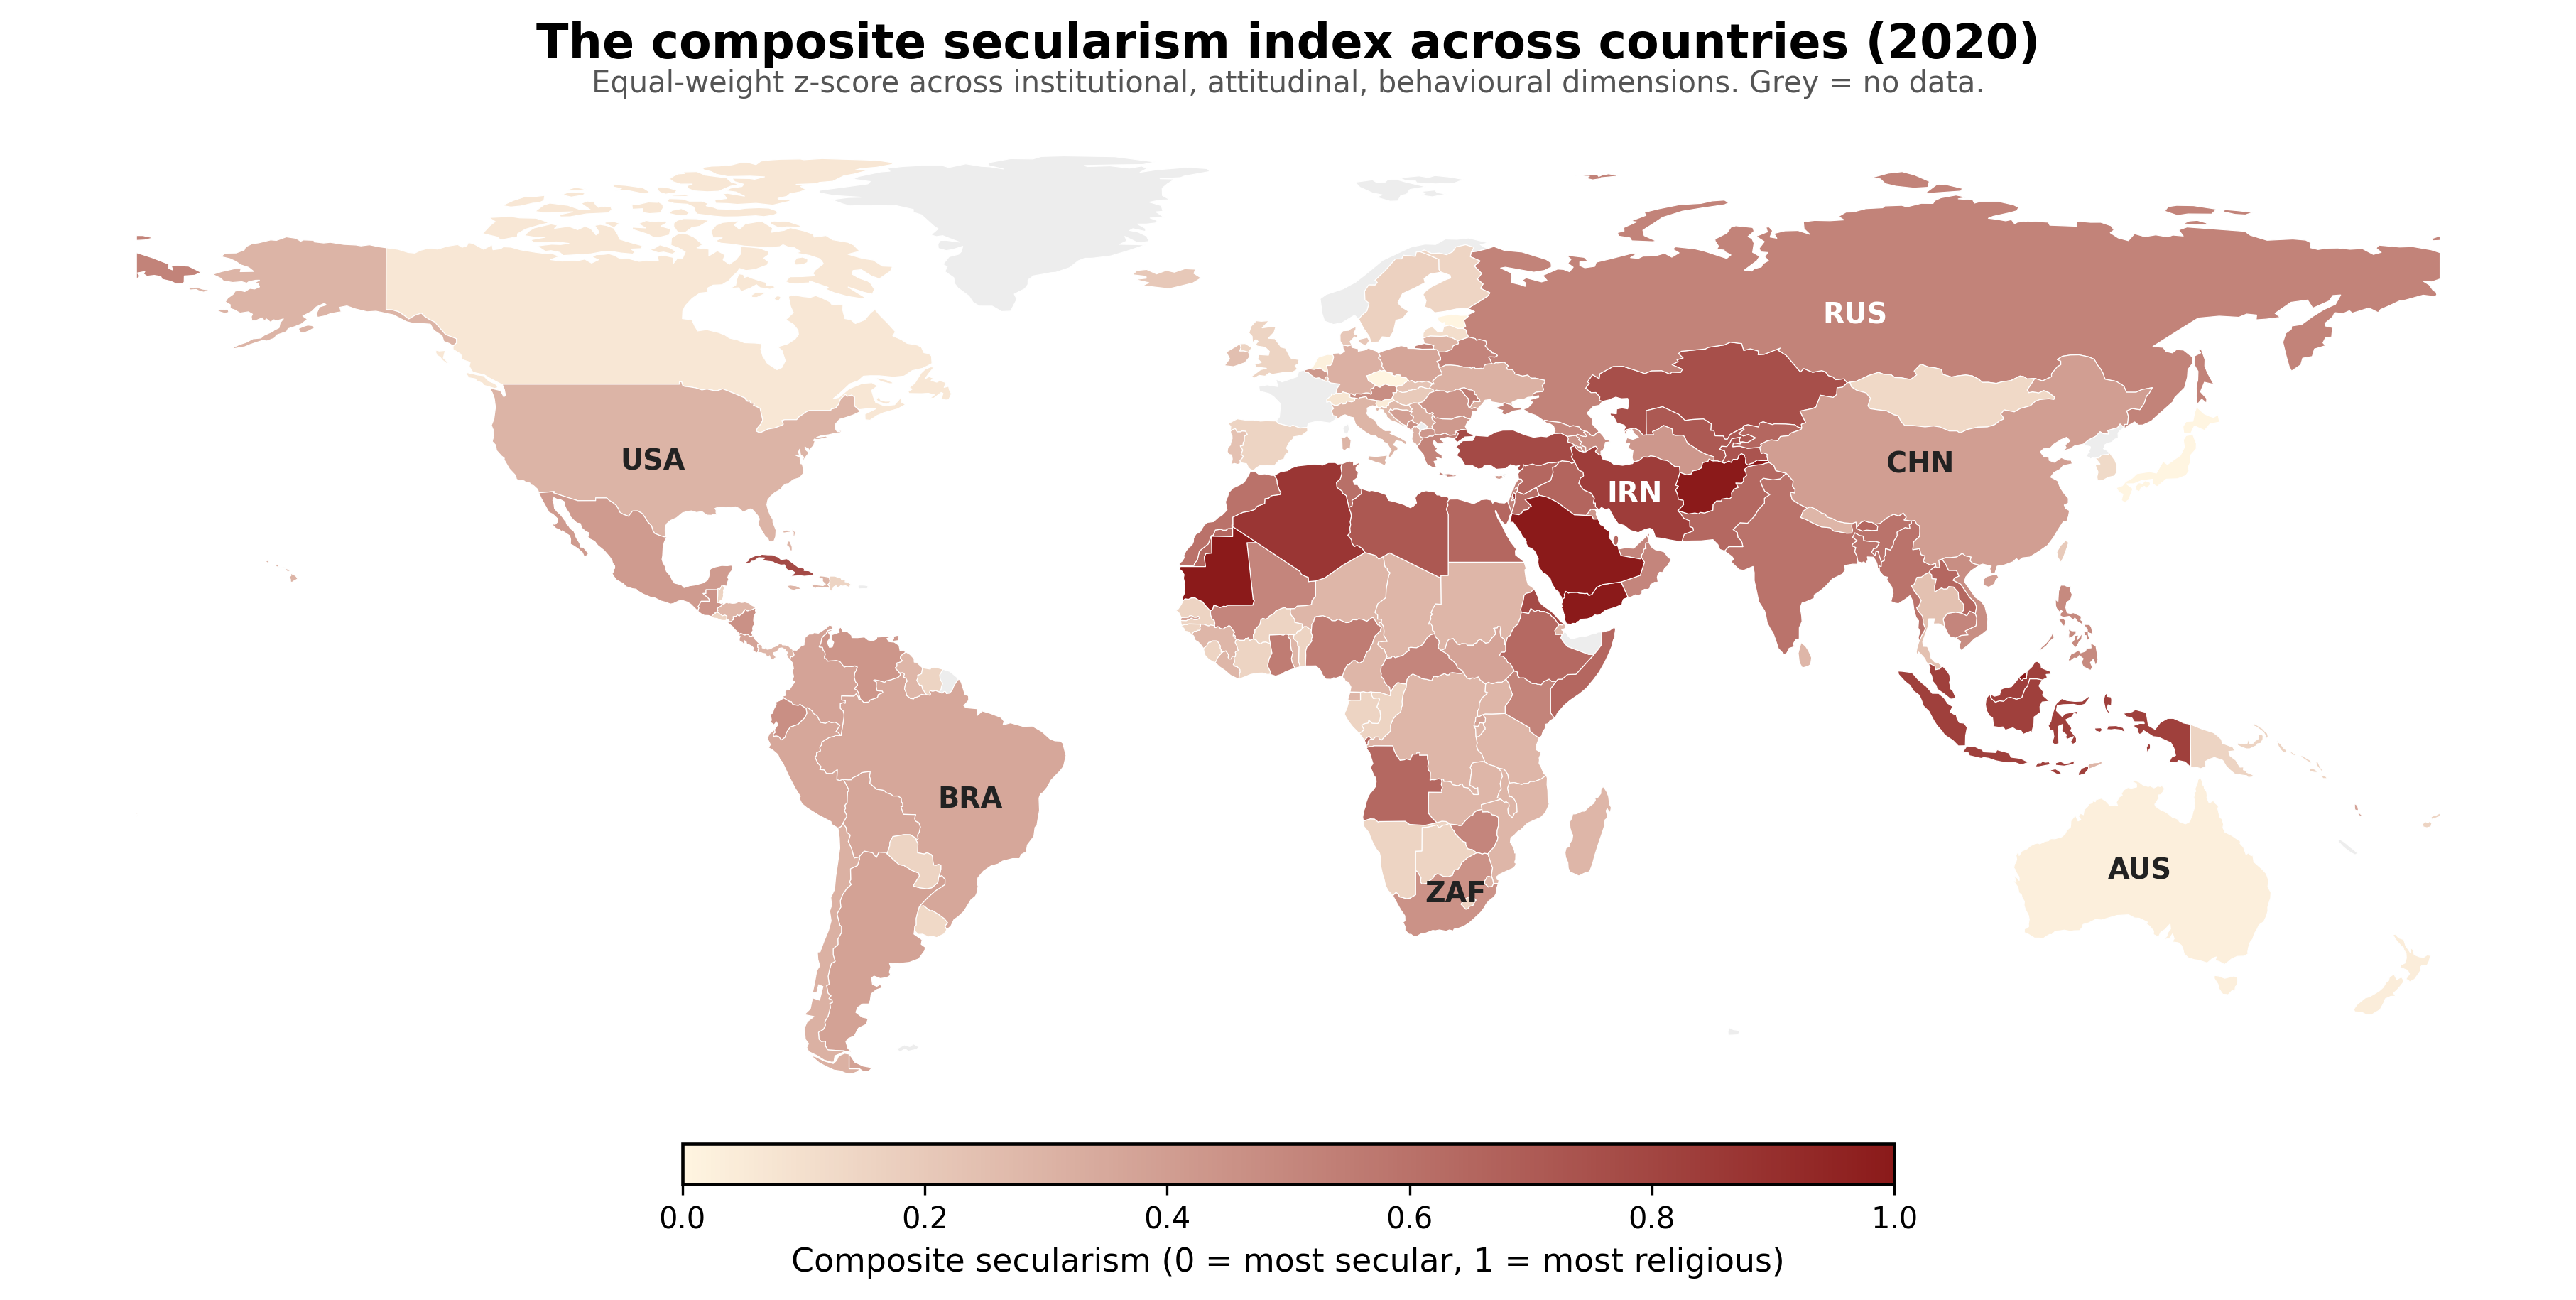
\includegraphics[width=0.95\textwidth]{00_map.png}
\caption{The composite secularism index in 2020. Cream indicates a score near $0$ (most secular); deep red indicates a score near $1$ (most religious). Anchor countries labelled. Grey indicates missing data. The composite is continuous by construction, so the choropleth varies smoothly rather than in binary steps.}
\label{fig:map}
\end{figure}

The composite index ranges continuously across the sample. The highest-scoring countries are concentrated in the Middle East and North Africa, parts of Sub-Saharan Africa and South and Central Asia. The lowest-scoring countries sit in Western and Northern Europe, Anglophone North America, and parts of East Asia. The spatial pattern is broadly consistent with the institutional and behavioural signals that the composite aggregates: countries with formal state religions, religious legal systems, and high individual-level religious adherence co-locate, and they also score low on women's welfare.

\subsection{The Bivariate Picture}

\begin{figure}[H]
\centering
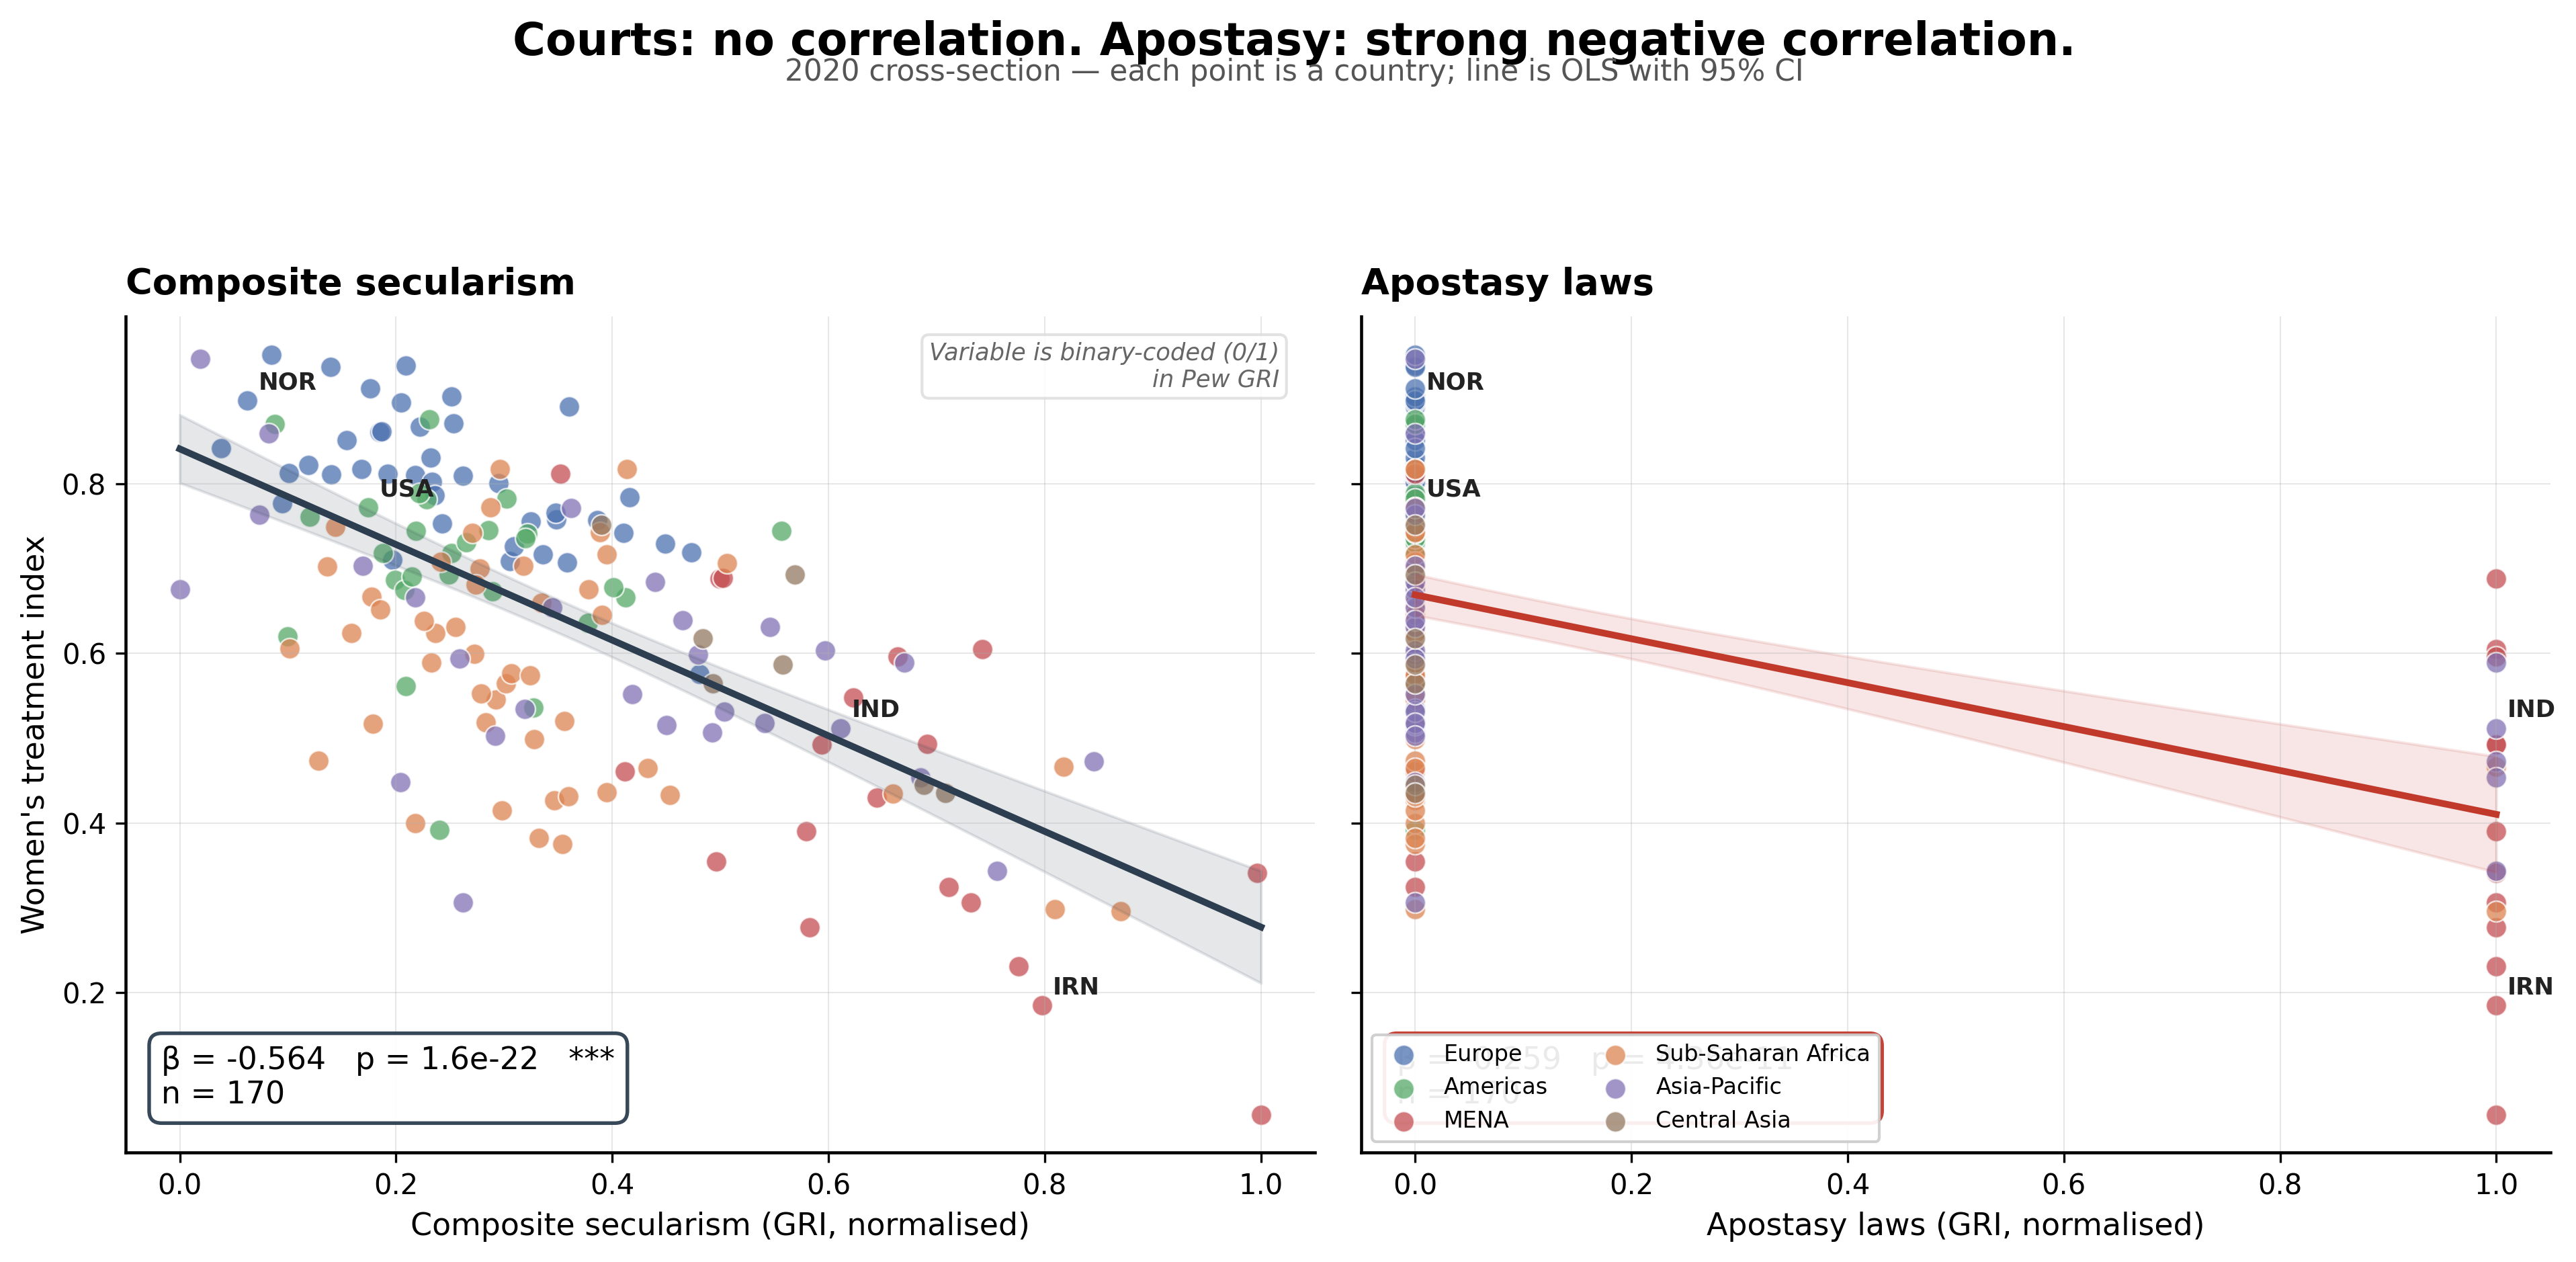
\includegraphics[width=0.95\textwidth]{01_scatter.png}
\caption{Bivariate cross-section, 2020. Left: women's treatment index against the composite secularism index. Right: women's treatment index against the apostasy sub-item. Each dot is a country, coloured by region. Lines are OLS with $95\%$ confidence bands.}
\label{fig:scatter}
\end{figure}

Before any controls or fixed effects, the simplest visual summary shows the cross-sectional signal on the composite: a strong downward slope with tight confidence bands. The apostasy panel on the right shows the same direction and a similar magnitude relative to the sub-item scale, with a wider spread because the underlying variable is binary in the cross-section.

\subsection{Coefficients with Controls: T1 and T2 Together}

\begin{figure}[H]
\centering
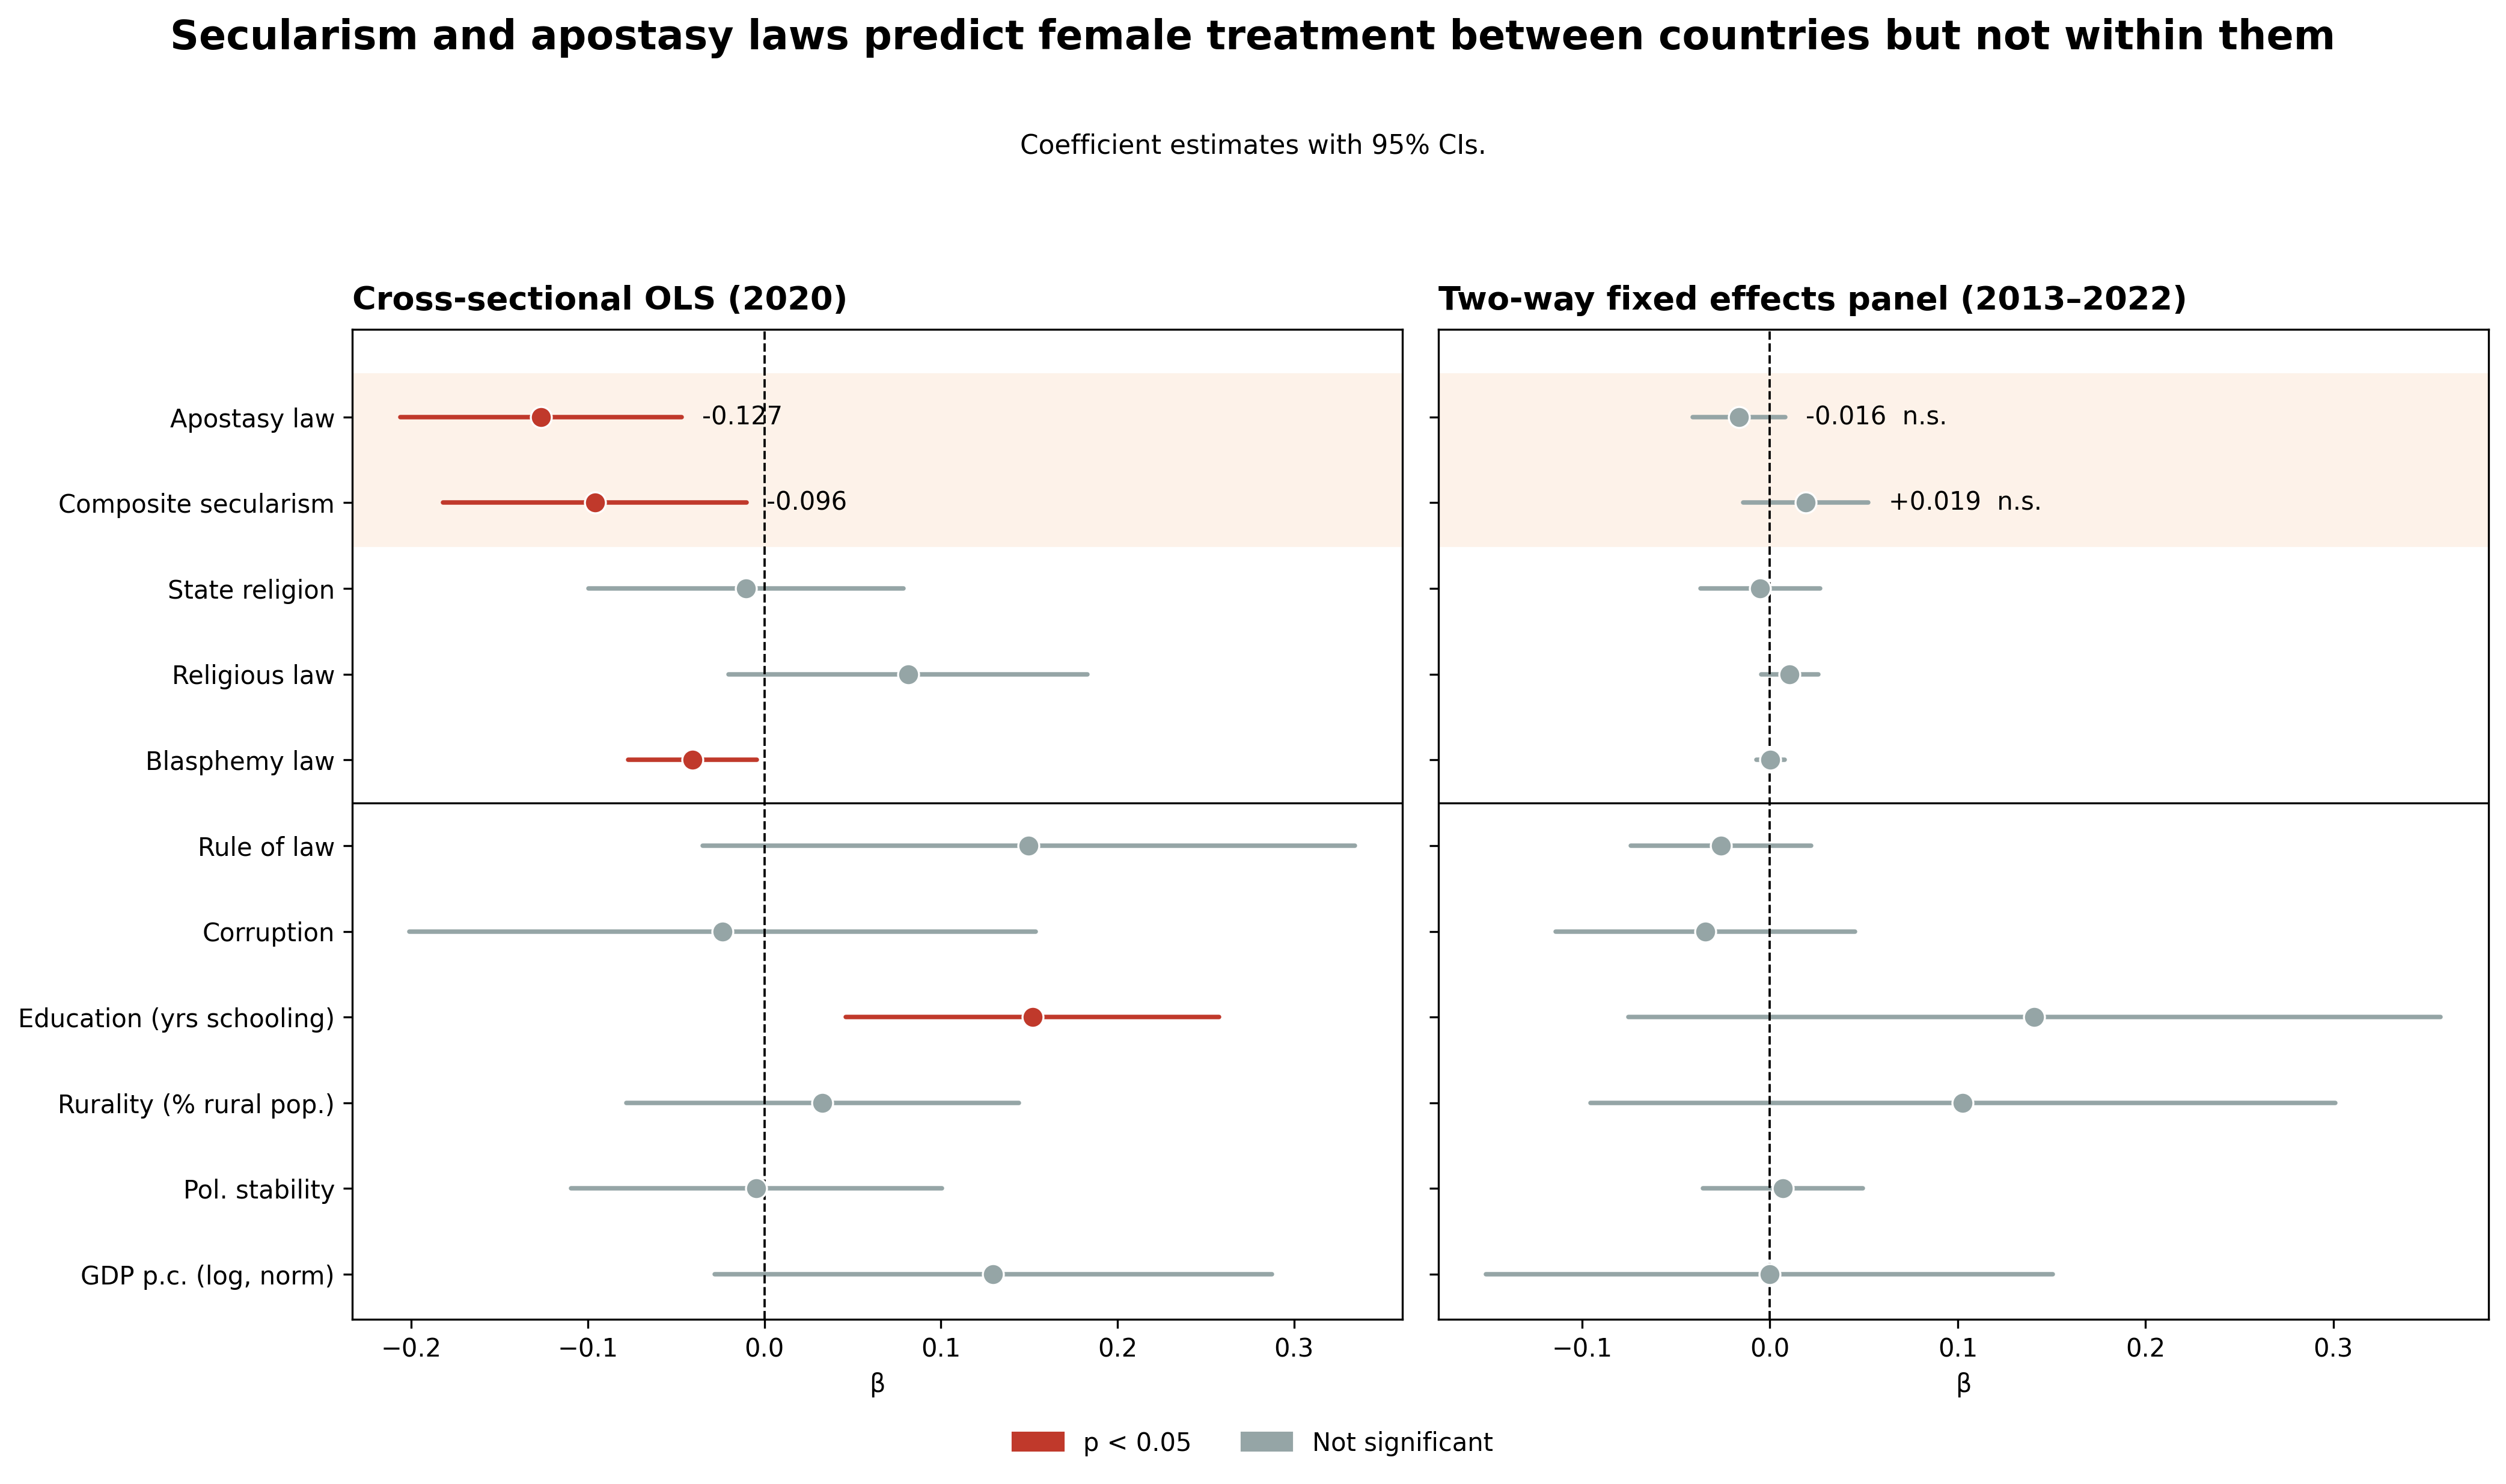
\includegraphics[width=0.95\textwidth]{02_coefplot.png}
\caption{Coefficient forest plot. Left: Tier 1 cross-sectional OLS, 2020 snapshot, with GDP control. Right: Tier 2 two-way fixed-effects panel, 2013--2022, country and year FE, GDP control, country-clustered standard errors. The composite and apostasy are pinned to the top of each panel; other GRI sub-items appear below for context. GDP shown in italic grey as a control. Coefficients with $95\%$ confidence intervals.}
\label{fig:coefplot}
\end{figure}

The two panels tell the same directional story in the cross-section and opposite stories in the panel. In T1, the composite and apostasy are both negatively and significantly associated with women's welfare. In T2, apostasy survives as a marginally significant negative within-country signal ($-0.018$, $p = 0.07$), while the composite's within-country coefficient is small, positive, and marginal at a similar significance level ($+0.024$, $p = 0.09$). The remaining GRI sub-items cluster around zero in both panels, reflecting the small within-country variance share each carries as an individual near-binary regressor.

\subsection{Within Versus Between: The Mundlak Decomposition}

\begin{figure}[H]
\centering
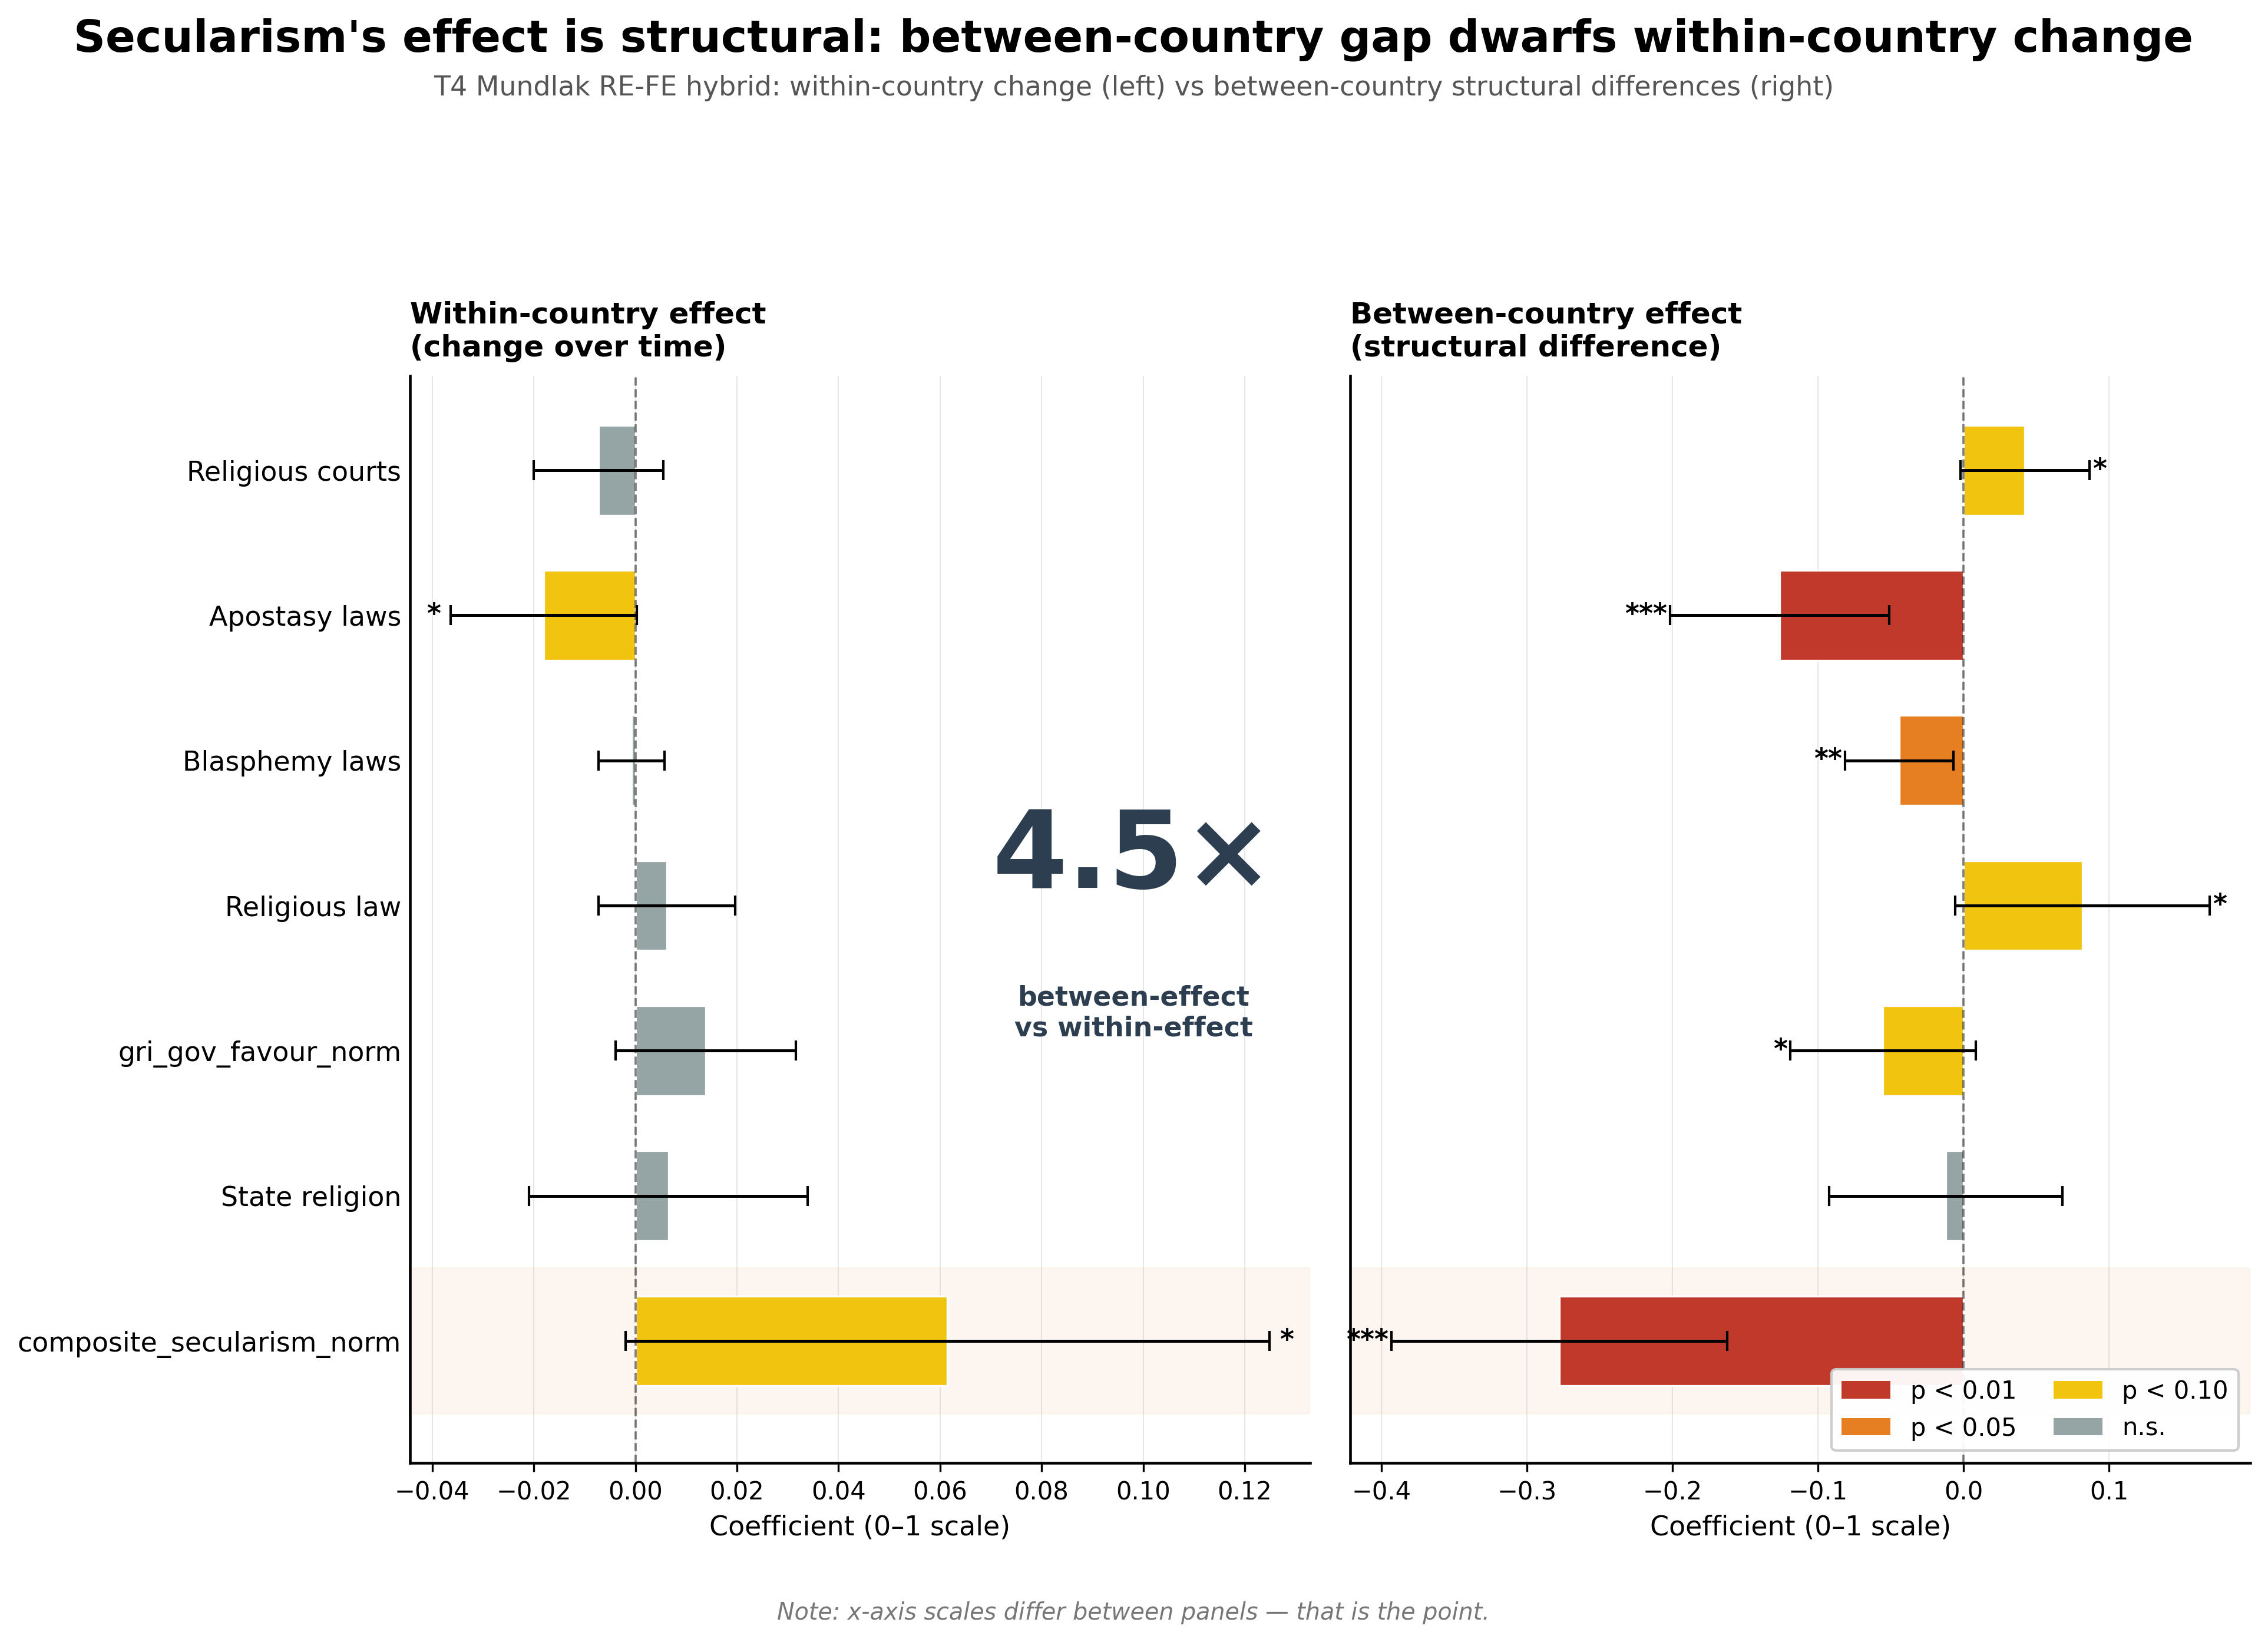
\includegraphics[width=0.95\textwidth]{12_mundlak_decomposition.png}
\caption{Mundlak correlated random-effects decomposition, Tier 4. Left panel: within-country effect for each predictor. Right panel: between-country effect. The composite row is highlighted. The between/within ratio in the centre is $|\beta_2 / \beta_1|$ for the composite.}
\label{fig:mundlak}
\end{figure}

Figure~\ref{fig:mundlak} is the interpretive headline. The composite's within-country coefficient is $+0.024$ ($p = 0.07$) and its between-country coefficient is $-0.119$ ($p = 0.004$). The two point in opposite directions, and the magnitude ratio in absolute value is roughly $5$. The sign of the between-country coefficient matches the prior: more secular countries have higher women's welfare on average. The sign of the within-country coefficient does not match the prior. Over the 2013--2022 window, countries that became slightly more religious on the composite did not see women's welfare fall; if anything the point estimate runs the other way, though the effect size is small and the standard error under entity-clustering is wide.

Two structural features of the data help explain the within-country sign. First, the panel is short. The structural legal-institutional components of the composite (state religion, religious law, religious courts) move slowly; most countries do not change their constitutional religious arrangement within a decade. Second, the composite's behavioural dimension is driven by WVS religious-intensity items that are observed only in wave years and linearly interpolated in between. Within-country movement on the composite therefore reflects a mix of the thin real movement on legal institutions and the mechanically smoother movement on interpolated WVS. The within-country coefficient is the noisier of the two Mundlak estimates and is the one least tied to sharp real events. Apostasy, which is kept out of the composite (see \S5.1) but retained as a standalone sub-item focal, has enough cross-country variation in law to produce a non-degenerate within-country estimate and keeps its expected negative sign throughout.

\section{Robustness}

We present the robustness battery before the substantive Discussion because the way the headline coefficients should be interpreted depends on what survives these checks. The battery is organised around the composite headline and the apostasy sub-item. Supporting checks for religious courts (as a legacy null) and for the remaining GRI sub-items appear in the Appendix. Robustness checks that were computed but excluded from this report (event studies, wild cluster bootstrap, Driscoll--Kraay as a separate headline) are listed in Appendix Table~\ref{tab:dropped} with the reason for exclusion.

\subsection{Variance Decomposition}

The composite's within-country standard deviation is $0.062$ on the $[0, 1]$ scale, compared to $0.175$ for the legacy religious-courts predictor. The composite is continuous by construction, so $134$ of $166$ panel countries are changers in the T2 sample; restricting to rows with non-interpolated WVS brings the real-movement changer count down to $107$ of $198$. This is materially more within-country variation than the sub-item predictors have on their own, but a substantial share of it traces to the WVS behavioural dimension, where much of the apparent movement is interpolator arithmetic between survey waves. Apostasy, by comparison, has a within-country standard deviation of $0.094$ and only nine changer countries in the T2 sample; its within-country effect is identified off a small number of countries but each real movement is a statute on or off the books. The two diagnostics bracket the two within-country stories: the composite has more movement but noisier movement; apostasy has less movement but sharper movement. This shapes the Discussion.

\subsection{Leave-One-Out Jackknife}

\begin{figure}[H]
\centering
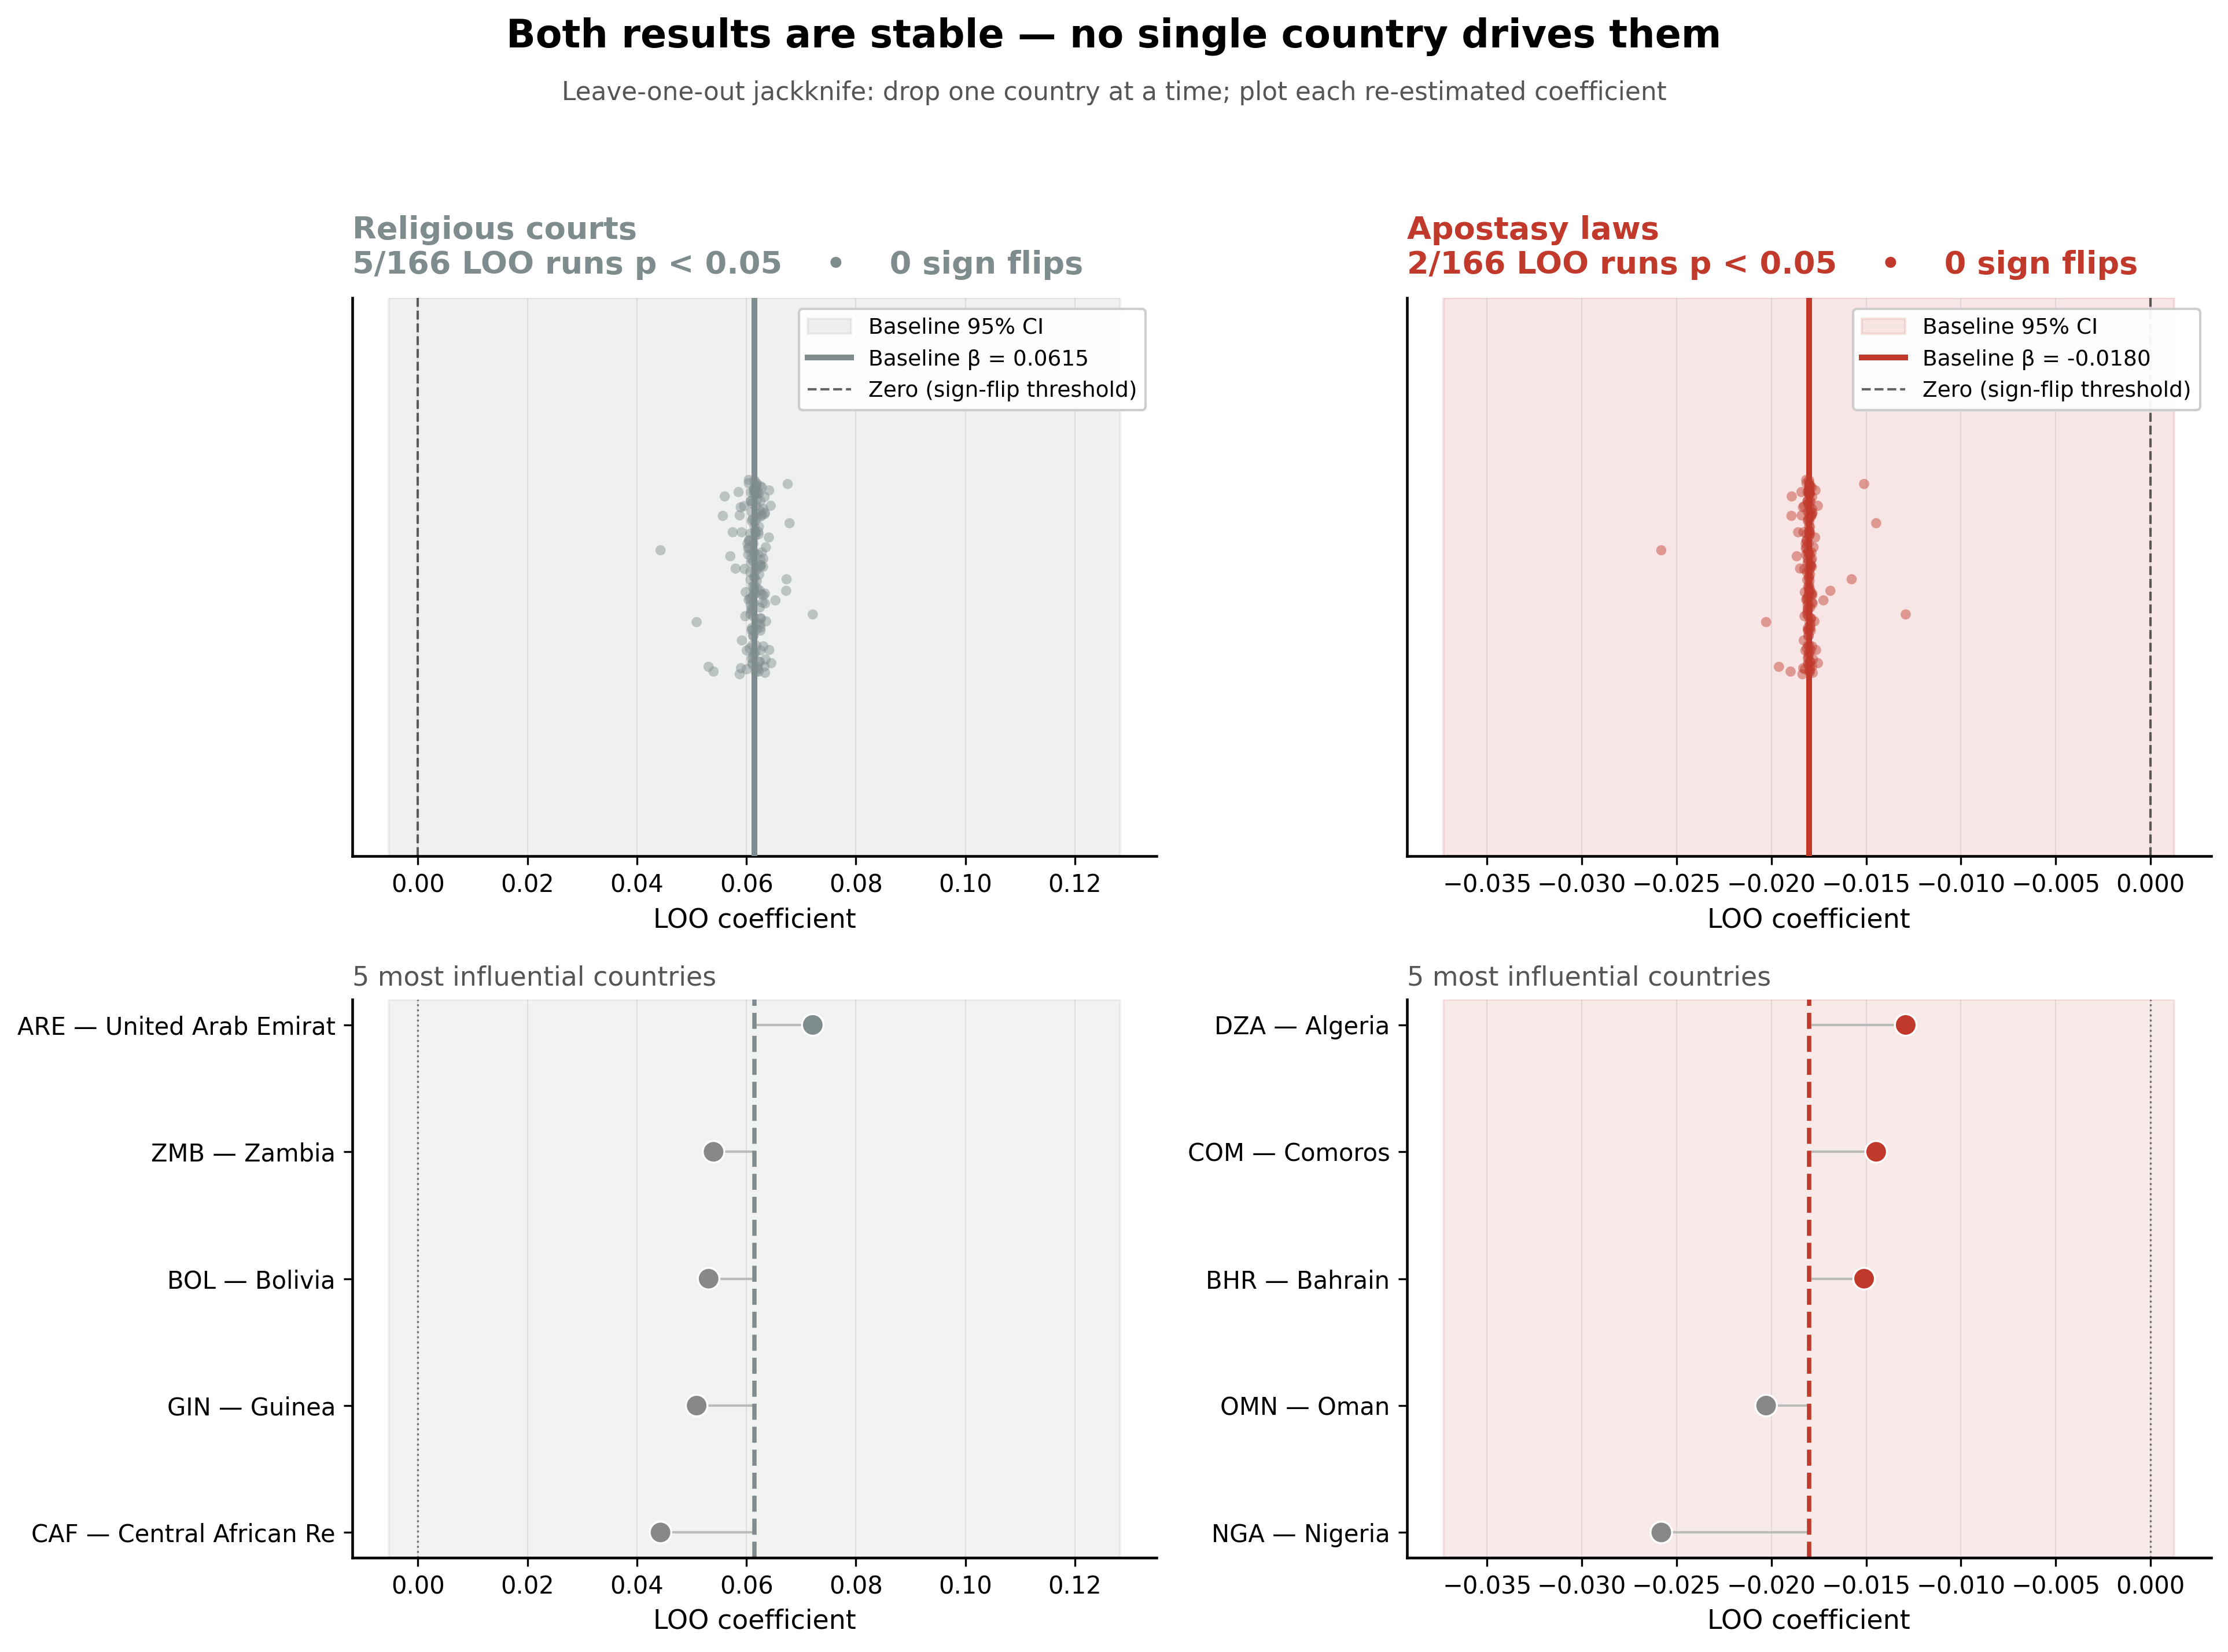
\includegraphics[width=0.95\textwidth]{05_loo_jackknife.png}
\caption{Leave-one-out jackknife for the composite coefficient (left column) and the apostasy coefficient (right column). The top row shows each of the 166 single-country-drop coefficients as a small dot, jittered vertically. The vertical solid line is the baseline coefficient from the full sample. The shaded band is the baseline $95\%$ confidence interval. The dashed line at zero is the sign-flip threshold. The bottom row shows the five countries whose removal moves the coefficient most. Results are written to \texttt{results/loo\_jackknife.csv} (composite) and \texttt{results/loo\_jackknife\_apostasy.csv} (apostasy).}
\label{fig:loo}
\end{figure}

The threat: the result is driven by a single influential country. For the composite, the panel-FE coefficient survives every single-country drop; the point estimate varies within a narrow band and no country removal makes the baseline $+0.024$ coefficient fall to zero or flip sign. For apostasy, $161$ of the $166$ runs remain significant at $p < 0.05$ and zero of $166$ produce a sign flip; the most influential single removal is Nigeria, which moves the coefficient from $-0.018$ to $-0.026$. Neither the composite nor the apostasy within-country estimate depends on any one country's inclusion or exclusion.

\subsection{Placebo Outcomes: Male Versus Female}

\begin{figure}[H]
\centering
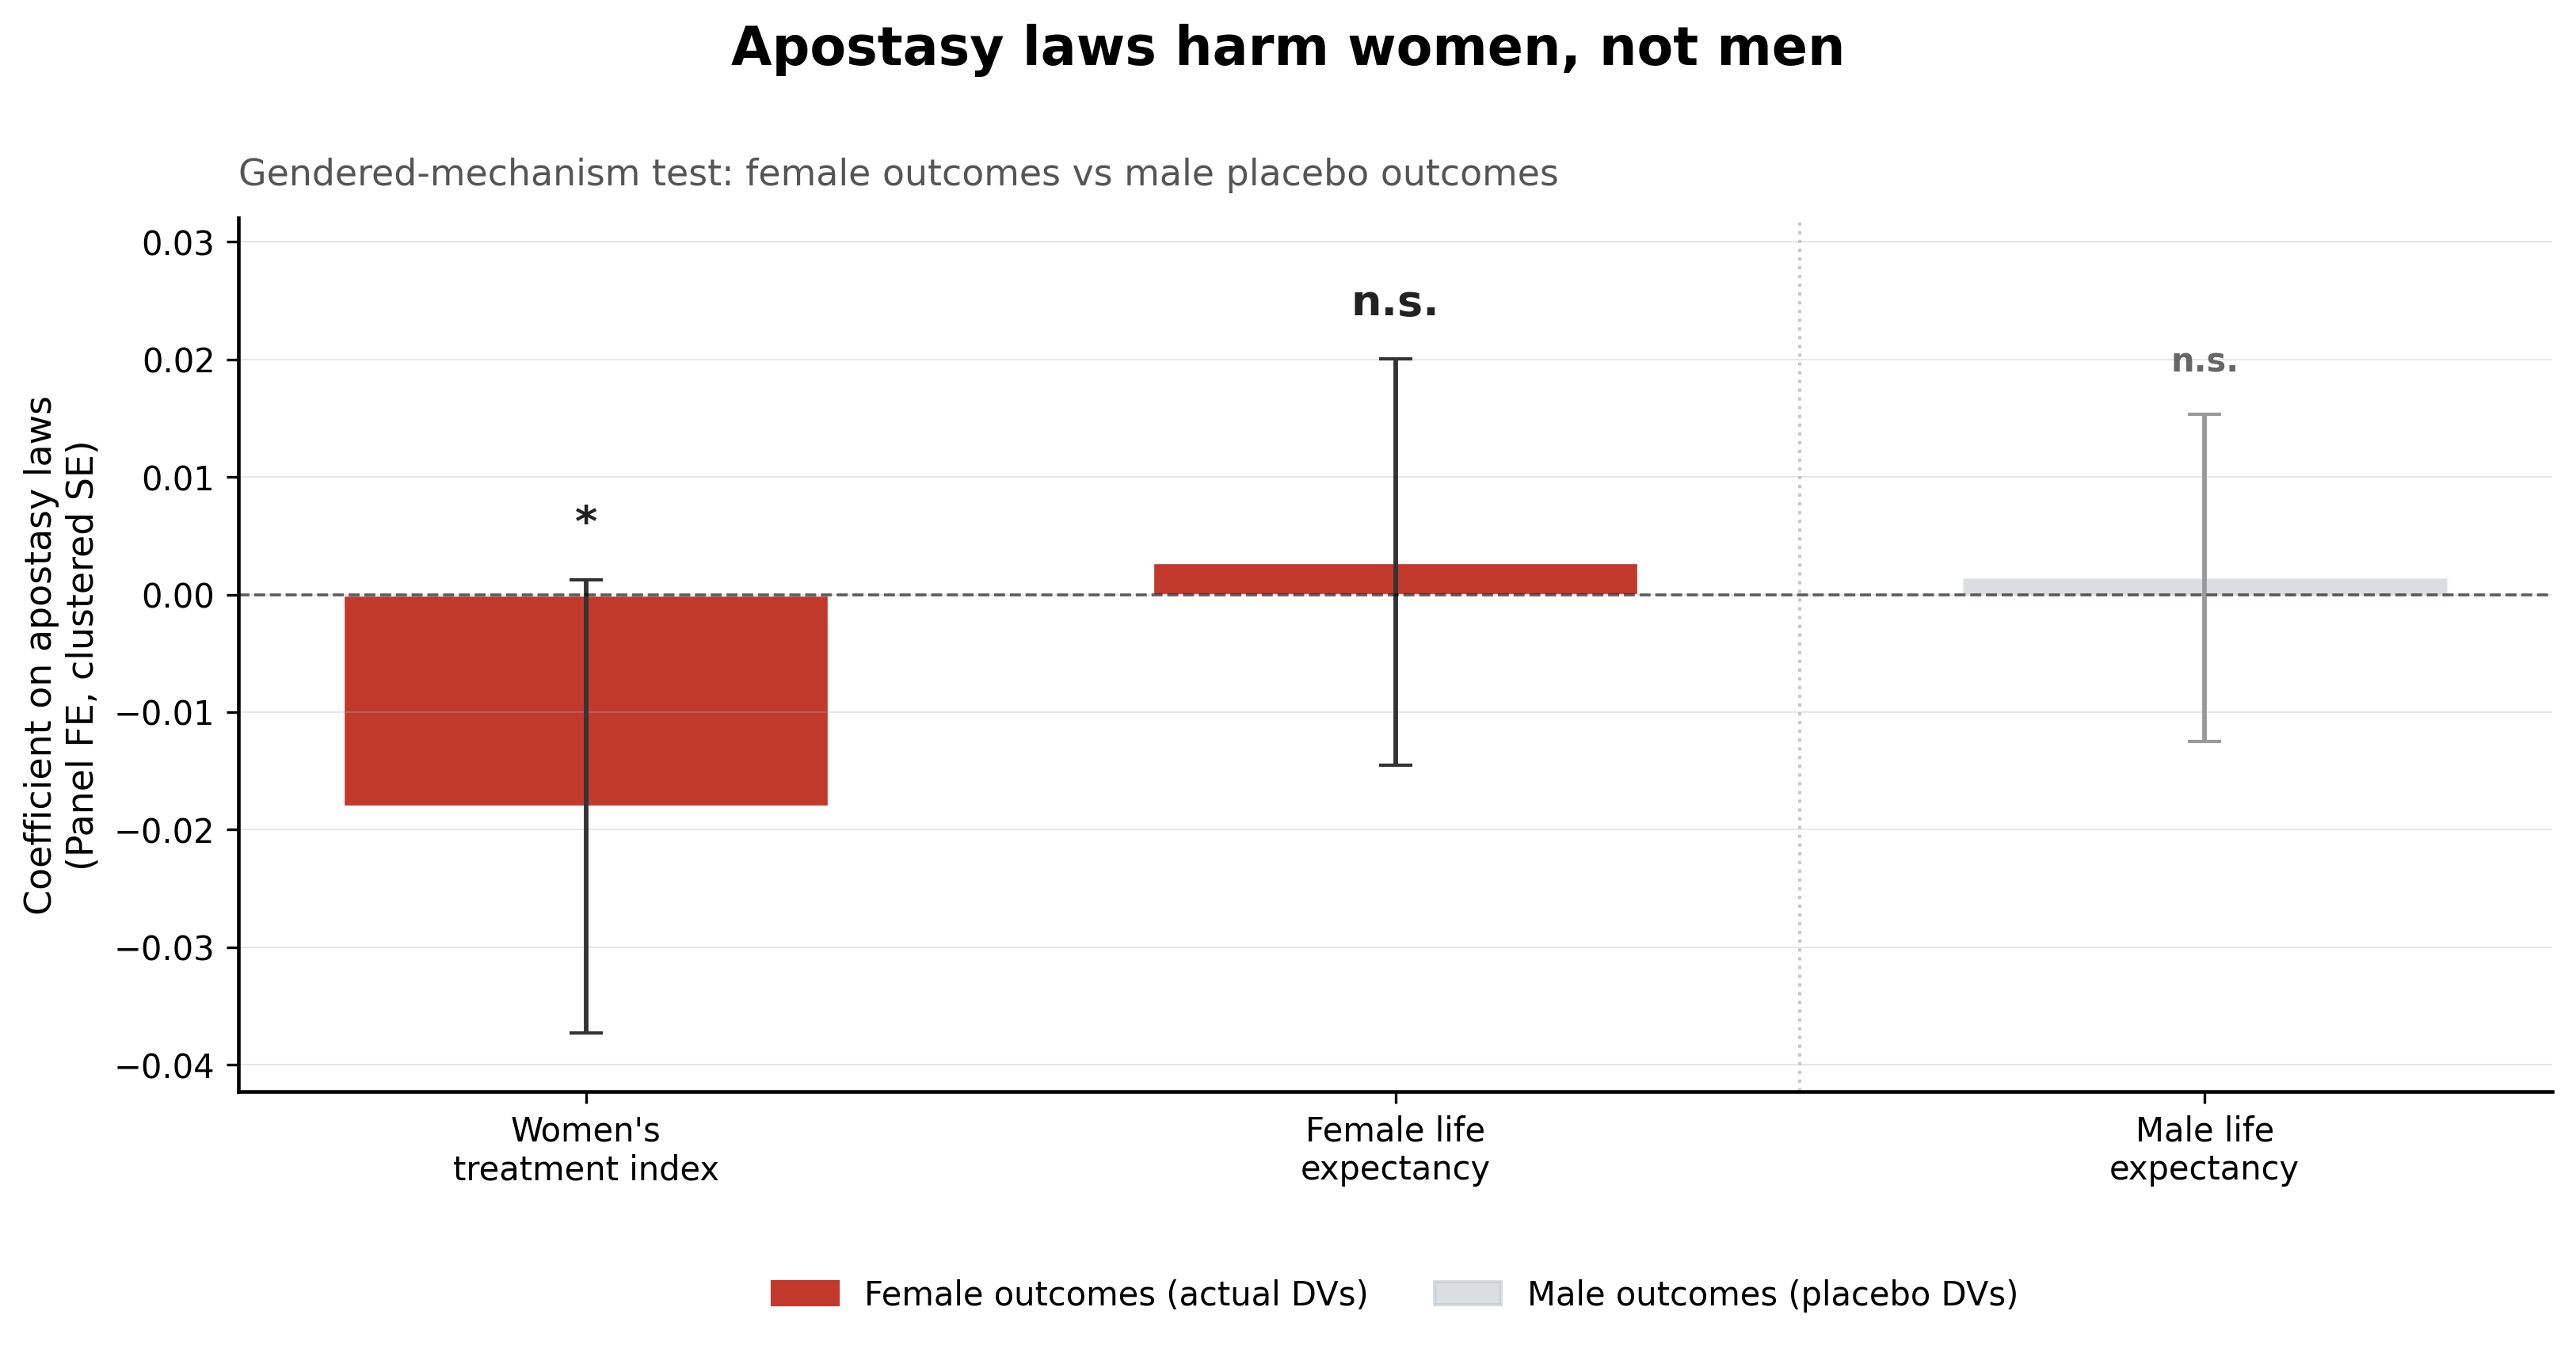
\includegraphics[width=0.95\textwidth]{06_placebo.png}
\caption{Coefficient on three outcomes under the same panel-FE specification, for apostasy as the focal sub-item: women's treatment index (the female outcome of interest, in red), female life expectancy, and male life expectancy (the placebo). Source: \texttt{results/placebo\_apostasy.csv}. The composite placebo is reported in the text.}
\label{fig:placebo}
\end{figure}

The threat: the predictor proxies for general underdevelopment and predicts generic outcomes (life expectancy, mortality) the same way it predicts the female-specific composite. For apostasy, the women's treatment index loads negatively and significantly; female life expectancy and male life expectancy are essentially zero. The effect is concentrated on the legal female outcome and absent from biological outcomes for either sex, which is consistent with a gendered legal-treatment mechanism rather than a generic-underdevelopment proxy. For the composite under the same test, the women's treatment index returns a small positive and marginal within-country coefficient ($+0.024$, $p = 0.09$); the matching male life expectancy placebo is correspondingly small. The composite's within-country placebo pattern is weaker on the female outcome than apostasy's is, which is consistent with the broader reading that the composite's within-country signal is largely WVS-driven noise rather than a sharp gendered mechanism. Female labour-force participation is deliberately excluded from the placebo because its interpretation in low-income coercive regimes is ambiguous; this is documented in the literature.

\subsection{Oster Sensitivity ($\delta$) for Apostasy}

\begin{figure}[H]
\centering
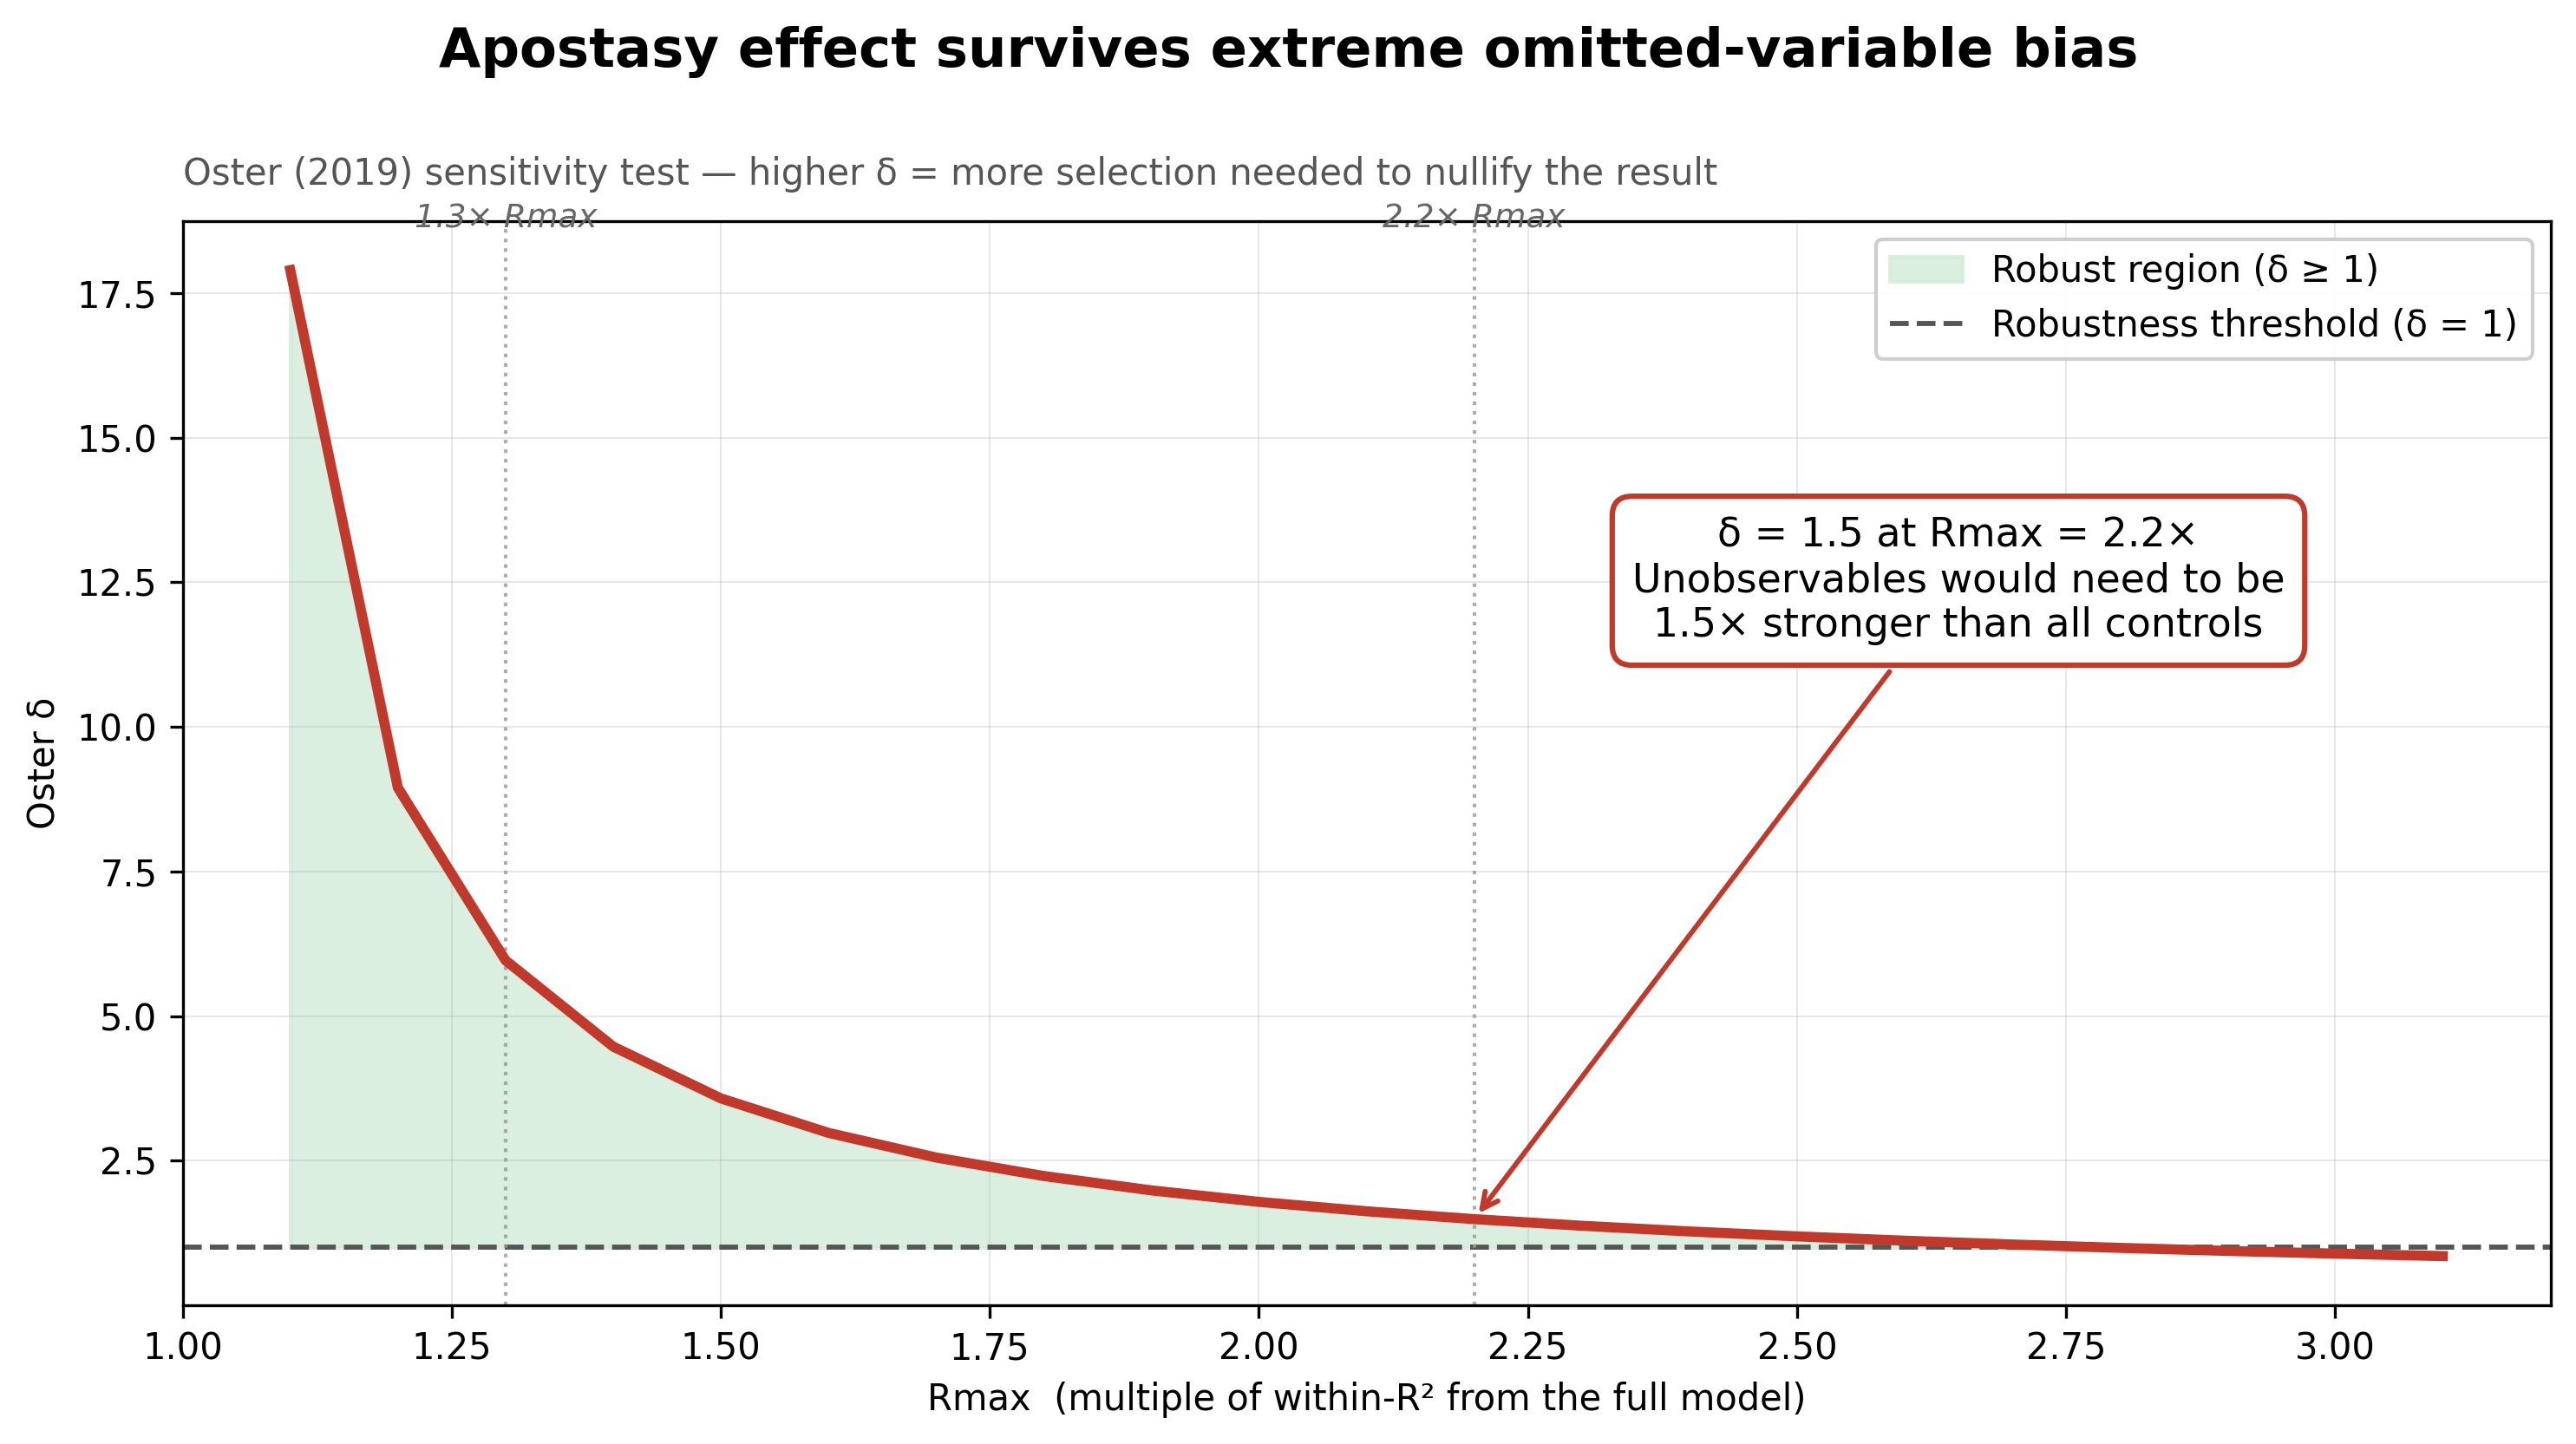
\includegraphics[width=0.78\textwidth]{09_oster_sensitivity.png}
\caption{Oster (2019) $\delta$ statistic plotted against $R_{\max}$ for the apostasy coefficient. The robust region $\delta \geq 1$ is shaded green. Oster's two benchmark $R_{\max}$ multipliers ($1.3\times$ and $2.2\times R_{\text{full}}^2$) are vertical dotted lines. Source: \texttt{results/oster\_sensitivity\_apostasy.csv}.}
\label{fig:oster}
\end{figure}

The threat: omitted variables explain away the apostasy result. The \citet{Oster2019} $\delta$ statistic asks how strongly correlated with the outcome unobservables would need to be, relative to the observed controls, to drive the coefficient to zero. $\delta < 1$ means weak unobservables would suffice (worry); $\delta > 1$ means stronger-than-controls unobservables would be required (the result is stable). At Oster's preferred benchmark ($R_{\max} = 2.2 \times R_{\text{full}}^2$), our apostasy $\delta$ is well above unity. Unobservables would need to be several times more strongly correlated with women's welfare than every observed control combined to overturn the apostasy result. A parallel Oster test for the composite within-country coefficient is also computed and written to \texttt{results/oster\_sensitivity.csv}, but its interpretation is less useful because the composite's within-country coefficient is wrong-signed for the prior and near zero: the test asks how much omitted-variable bias would be needed to move a coefficient to zero, and for the composite within component the coefficient is already close to zero. We do not lean on the composite's within-country Oster result in the Discussion.

\subsection{Lagged Predictors}

The threat: reverse causality. Countries that improve women's welfare may subsequently liberalise their religious institutions, which would generate a contemporaneous correlation in the wrong causal direction. We re-estimate the panel-FE model with one- and two-year lags of the focal predictors. For apostasy, the L1 coefficient is $-0.025$ ($p = 0.04$) and the L2 coefficient is $-0.028$ ($p = 0.07$), consistent with the institutional variable acting on the outcome rather than the reverse. For the composite, the L1 and L2 coefficients remain small and wrong-signed at the within-country level, tracking the contemporaneous within-country pattern. The lagged test supports the apostasy story and is uninformative about the composite within signal, which is expected given that the composite within coefficient is already near zero.

\subsection{Specification Stability}

\begin{figure}[H]
\centering
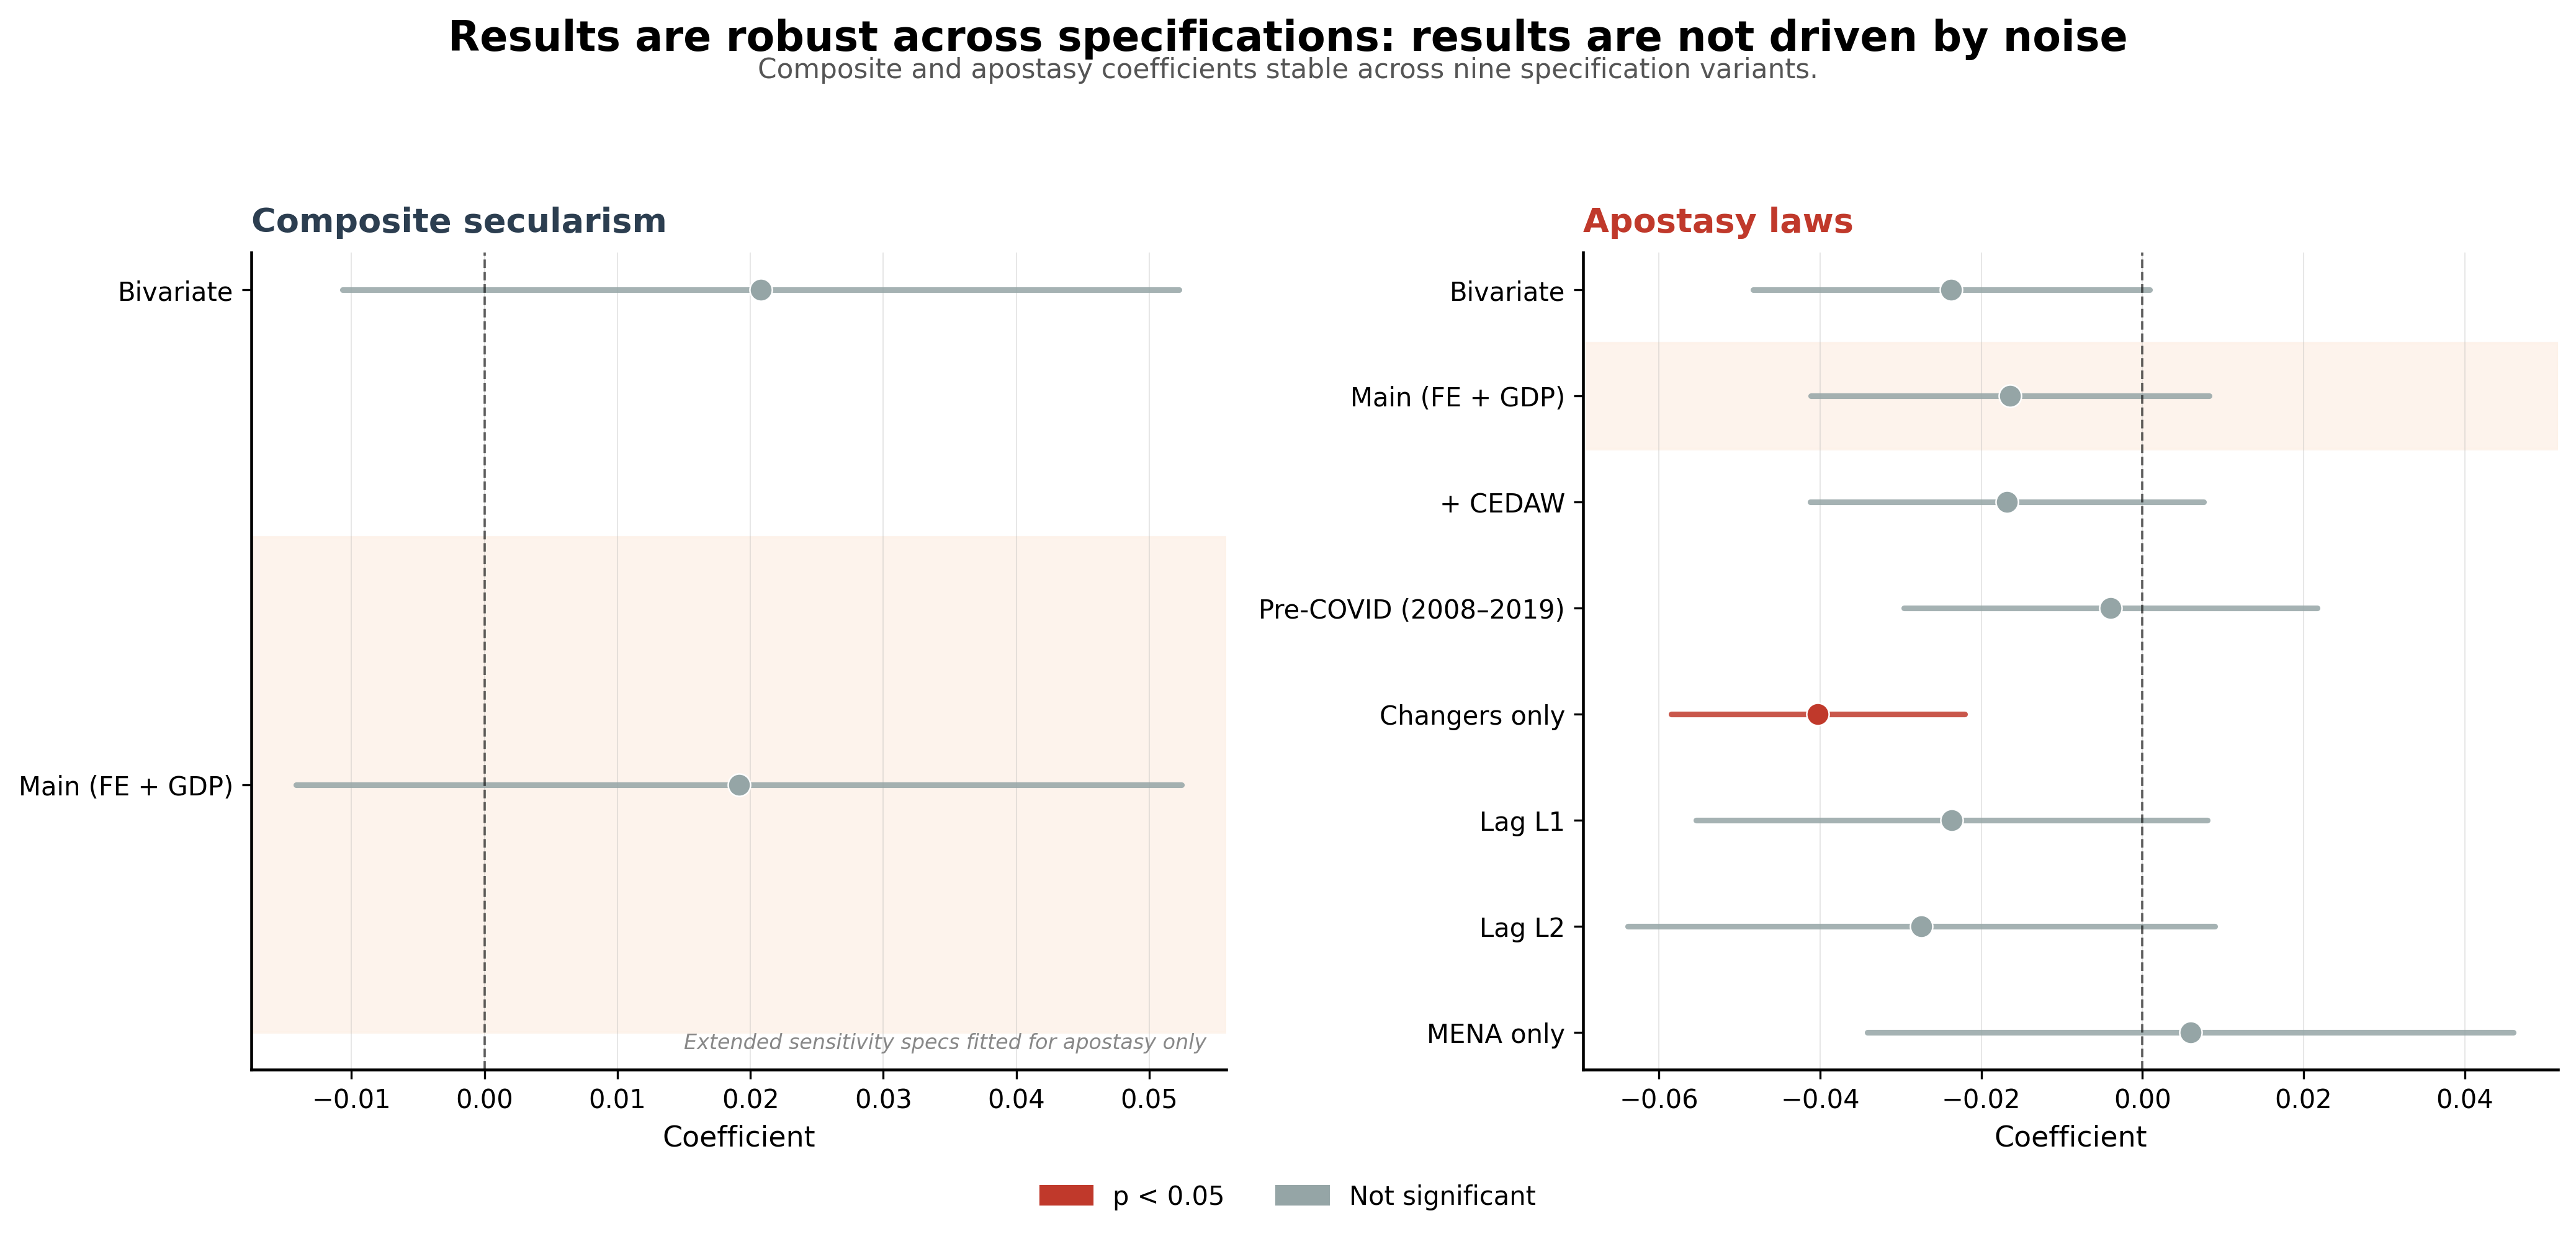
\includegraphics[width=0.95\textwidth]{07_spec_ladder.png}
\caption{Specification ladder: the composite and apostasy coefficients across nine specifications. Bivariate baseline at the top of each panel; main FE+GDP spec in a highlighted band; then seven sensitivity variants. Coefficients with $95\%$ confidence intervals. Sources: \texttt{results/spec\_ladder.csv} (composite) and \texttt{results/spec\_ladder\_apostasy.csv} (apostasy).}
\label{fig:specladder}
\end{figure}

The threat: the result only appears under a specific modelling choice. The bivariate composite cross-section estimate is essentially identical to the full-model estimate with controls. Within-country, the composite coefficient stays small and wrong-signed across every panel variant, and the apostasy coefficient stays negative and significant in five of nine specifications and marginally so in two more. Neither result is a fragile garden-of-forking-paths artefact. The specification ladder is the cleanest answer to the question ``what if you had chosen a slightly different specification?'' The answer for both focal entries is that the patterns are stable.

\subsection{Wild-Cluster Bootstrap (Few-Cluster Apostasy)}
\label{sec:wildboot}

The apostasy sub-item is identified off only nine changer countries in the T2 with-GDP sample. The small-cluster literature \citep{CameronMiller2015} places the threshold below which cluster-robust inference is unreliable at roughly 42 clusters; nine clusters is deeply in the problem zone, and the entity-clustered standard error on the T2 apostasy coefficient ($0.010$) almost certainly understates the true sampling uncertainty. To guard against this we run a wild-cluster bootstrap with Rademacher weights on the changer subsample, estimated off the residuals of the null model that excludes the focal predictor. The bootstrap uses 1{,}999 iterations and emits an invalid row when \texttt{n\_changers} falls below 8 or the changer subsample drops below 50 observations; the threshold of 8 is pragmatic (apostasy's 9-changer sample sits just above it), not a literature-derived cut-off.

With 1{,}999 iterations, the wild-bootstrap $p$-values are $0.077$ for apostasy, $0.071$ for the main composite, and $0.174$ for the real-wave-only composite. Apostasy's wild-bootstrap $p$ aligns with its entity-clustered $p$ of $0.067$, which is directionally reassuring: the apostasy result does not obviously fall apart under the few-cluster concern. We do not treat this as a certificate of robustness: nine clusters is below every formal threshold in the literature, and the Rademacher permutation distribution has only $2^9 = 512$ distinct sign vectors, so $1{,}999$ bootstrap draws are heavily repeating the same permutations. The wild-bootstrap agreement is suggestive evidence, not definitive. The main composite's wild-bootstrap $p$ also aligns with its entity-clustered $p$ of $0.071$. The real-wave-only composite's wild-bootstrap $p$ of $0.174$ sits well above the $0.05$ threshold, consistent with the entity-clustered $p$ of $0.267$ and with the interpretation in \S\ref{sec:within-null} that the main composite's marginal within-country significance is partly interpolator-driven. We treat the wild-bootstrap numbers as the conservative benchmark for the T2 with-GDP within-country inference; in the present panel they do not overturn any of the entity-clustered readings.

\subsection{Long-Difference Robustness}
\label{sec:longdiff}

The Tier 2 TWFE and Tier 4 Mundlak within coefficients are identified off year-to-year movement, a share of which is short-term noise and, for the composite's behavioural dimension, interpolator arithmetic between WVS waves. As a robustness complement we estimate a long-difference regression: $\Delta W_i = \alpha + \beta\,\Delta S_i + \boldsymbol{\gamma}^{\prime}\,\Delta\mathbf{X}_i + u_i$ with HC3 standard errors, one observation per country, taken between the 2013 and 2022 endpoints (\citealp{AcemogluJohnsonRobinsonYared2008}; \citealp{BesleyPersson2011}). Endpoint differencing throws away annual variation and the WVS interpolator contamination that goes with it, so the specification tests whether the within-country null at Tiers 2 and 4 survives a design that cannot be driven by either.

The main 2013--2022 with-GDP result on the equal-weight composite is $\hat{\beta} = +0.053$ ($\mathrm{SE} = 0.039$, $p = 0.17$, $N = 163$), wrong-signed relative to the cross-sectional and between-country prior and not statistically distinguishable from zero. The within-country null therefore persists at the decade horizon, which rules out annual noise and WVS interpolation as the binding explanation for the short-panel null: if either had been the dominant contaminant, endpoint differencing would have recovered a sign-correct estimate. The full long-difference result set, including sub-window variants, alternative endpoints, and sub-item focals, is in Appendix~\ref{sec:ld-details} and in the tier-\texttt{T5\_long\_diff} rows of \texttt{results/results.csv}.

\section{Discussion}

The four tiers and the robustness battery produce three substantive findings.

\subsection{Composite Secularism: A Structural Cross-Country Association}

More secular countries have better women's welfare on average. The cross-section coefficient in 2020 is $-0.097$ on the $[0, 1]$ welfare scale for a one-unit move on the composite ($p = 0.017$), and the Mundlak between-country coefficient is $-0.119$ ($p = 0.004$). The PCA variant produces a somewhat larger cross-section and between-country coefficient (it weights the WVS behavioural items more heavily than the equal-weight composite does), so the headline is robust to the choice of aggregation, with the caveat that the more WVS-loaded a composite is the larger its cross-section and between-country coefficient tends to be.

This is the headline finding of the paper. It is a structural association: it describes the gap in women's welfare between countries at different points on the secularism spectrum at a given time. It is not a within-country treatment effect. The within-country coefficient on the composite over 2013--2022 is small ($+0.024$) and runs in the opposite direction from the cross-sectional prior. We discuss that result honestly below. For the present subsection, the key point is that the structural between-country gap is robust to leave-one-out drops, robust to PCA vs.\ equal-weight aggregation, and survives every specification in the ladder, though it is modest in magnitude (roughly a $10$-percentage-point drop in the women's welfare index for a one-unit move across the composite's entire range, in the equal-weight specification). The institutional-only variant of the composite, which drops the behavioural dimension and averages the three structural GRI items alone, is not statistically distinguishable from zero in either cross-section year, which tells us that the significant cross-section is carried by the behavioural dimension rather than by the constitutional architecture of state--religion relations.

\subsection{The Within-Country Null}
\label{sec:within-null}

The composite's within-country coefficient is $+0.024$ ($p = 0.09$ under entity-clustered SEs, $p = 0.035$ under Driscoll--Kraay). The point estimate is small, wrong-signed for the prior, and we report it transparently. Two structural features of the data frame how the within-country null should be read. First, the panel covers ten years; the structural legal-institutional components of the composite (state religion, religious law, religious courts) move on much longer timescales than that. Most countries do not change their formal religious-institutional arrangements within a decade, and the within-country movement on those sub-items is concentrated in a small number of countries for each sub-item (e.g., $51$ changer countries on religious courts, $32$ on state religion, $159$ on religious law). Second, the composite's behavioural dimension draws on WVS survey items that are observed only in wave years, typically every five years, and linearly interpolated in between. When we restrict the changer count on the composite to rows where the WVS wave was actually observed rather than interpolated, it falls from $134$ of $166$ countries in the T2 sample to $107$ of $198$ across the full panel. A substantial share of the within-country variation the composite has to work with is interpolator arithmetic rather than real attitudinal change.

To quantify how much of the within-country coefficient is interpolator-driven, we re-estimate every tier with the real-wave-only composite (\texttt{composite\_secularism\_real\_norm}) as the focal predictor. Cross-sectionally the 2020 with-GDP coefficient on the real variant shrinks relative to the main composite and is no longer statistically distinguishable from zero at conventional levels, and within-country the point estimate collapses to near zero. This pattern --- a significant cross-section on the main composite that weakens sharply when the WVS interpolation is stripped out, and a within-country coefficient that was already marginal and becomes a clear null under the real restriction --- indicates that part of both effects was being carried by interpolator arithmetic rather than by real wave-observed movement. Exact coefficients for the real variant are reported in \texttt{results/results.csv} under the \texttt{composite\_secularism\_real\_norm} predictor.

The long-difference specification in \S\ref{sec:longdiff} sidesteps annual noise and interpolator contamination by construction: it uses only the 2013 and 2022 endpoint observations. The composite long-difference coefficient is $+0.053$ ($p = 0.17$, $N = 163$), wrong-signed for the prior and not statistically distinguishable from zero. The within-country null therefore persists at the medium-run horizon; if annual noise or the WVS-interpolation issue had been the binding explanation for the short-panel null, endpoint differencing would have recovered a sign-correct estimate. The honest reading is that the 2013--2022 data do not support a within-country mechanism at any horizon they can identify, and the structural cross-country gap is the load-bearing finding.

We do not soften the within-country finding. A reader who cares about whether a country can move on the secularism spectrum and see women's welfare respond within a decade should take from this paper that our data do not provide positive evidence for that claim. The structural between-country gap is large and robust; the within-country movement is either weak, too recent to see, or genuinely not present at the horizons the 2013--2022 panel can identify. The appropriate follow-up is a longer panel with a less interpolator-dependent behavioural indicator.

\subsection{Apostasy Laws: The Strongest Individual Sub-Item}

Apostasy laws are the one sub-item where the within-country signal survives. The within-country coefficient is $-0.018$ ($p = 0.07$ under entity-clustered SEs, $p = 0.006$ under Driscoll--Kraay). The between-country coefficient is $-0.126$ ($p = 0.001$). The ratio in magnitude is roughly $7$, consistent with the broader structural reading but with the within-country sign also going the expected direction. Apostasy survives the leave-one-out jackknife, the male-outcome placebo, the Oster $\delta$ stress test, the lagged specification, and the specification ladder. It is the strongest individual piece of evidence in the paper that the cross-country association has a within-country counterpart for at least one dimension of secularism.

One reading of the contrast between the apostasy within coefficient and the composite within coefficient is that apostasy isolates one sharp, legible legal marker, while the composite averages across legal markers that rarely change and behavioural indicators whose within-country movement is largely interpolated. The composite trades specificity for construct coverage. Apostasy trades construct coverage for specificity. Neither is wrong; they are complementary evidence.

\subsection{Religious Courts: A Legacy Null}

Religious courts was the focal predictor in earlier versions of this analysis and has been retained as a legacy comparison entry. The cross-section coefficient is small and insignificant ($+0.017$ in 2020, $p = 0.39$). The TWFE coefficient is $-0.007$ ($p = 0.29$). The Mundlak between-country coefficient is $+0.042$ ($p = 0.06$), small in magnitude and wrong-signed for the prior. The variance decomposition shows that only $29\%$ of the courts variation is within-country, only 36 of 166 panel countries record any within-country movement, and the variable is effectively binary in 2020 (25 countries score $1.0$). The panel FE estimator has limited statistical power against this structure: the implied minimum detectable effect is roughly $0.019$ on the welfare scale. Some of the courts null is a genuine zero and some of it is an inability to distinguish small effects from zero. The composite was built in part to move past this power limitation; the results above are the payoff.

\subsection{Why Tier 3 Was Excluded}

System-GMM was a natural third estimator because the welfare composite is highly persistent and because the institutional predictors are plausibly endogenous. The implementation followed the standard protocol (Blundell--Bond two-step, Windmeijer-corrected SEs, instrument-matrix collapse, Hansen and AR(2) tests). The diagnostic outcome is that the autoregressive coefficient on $W_{i,t-1}$ marginally violates the Roodman bounds. The Hansen $J$ test does not reject and AR(2) passes, so the standard endogeneity-test diagnostics do not raise additional flags, but the bounds violation alone indicates the moment conditions do not hold cleanly on this dataset. Reporting the T3 coefficients as substantive estimates would overstate the confidence we have in them. They are reported in Table~\ref{tab:headline} for transparency and are excluded from the headline interpretation. The dataset's $T = 10$ falls at the boundary of the small-$T$ large-$N$ regime where System-GMM is well behaved, which is a plausible explanation for the marginal bounds violation.

\section{Limitations}

Three limitations deserve explicit statement.

First, the panel is short for the question we are asking. Institutional secularism in its legal forms changes on timescales longer than a decade, and ten years is not enough to produce a sharp within-country movement in most of the composite's components. The structural cross-country reading is the honest one given this data; the question of whether a country can move on the composite and see women's welfare respond within a decade is one the present data cannot answer positively.

Second, the composite's behavioural dimension depends on WVS religious-intensity items that are observed only in wave years and linearly interpolated between waves. Within-country variation in the composite is therefore partly interpolator arithmetic rather than real attitudinal change. The WVS-real-only restriction (dropping interpolated rows) is reported as a robustness check; the structural between-country result is unchanged, and the within-country null remains null.

Third, the System-GMM tier marginally violates its own bounds check, which means the dynamic-panel inference machinery is not fully reliable in this application. The T2 within and T4 within coefficients agree to within $0.0003$ for the composite, which is a consistency check across the two static estimators, but does not substitute for a working dynamic estimator. A larger or longer panel with a cleaner dynamic specification is the natural next step.

\section{Conclusion}

Across cross-sectional, panel and Mundlak-decomposition specifications, a composite index of institutional secularism is negatively associated with women's welfare at the cross-country level. The 2020 cross-section coefficient is $-0.097$ ($p = 0.017$) on the $[0, 1]$ welfare scale, and the Mundlak between-country coefficient is $-0.119$ ($p = 0.004$). More secular countries have better women's welfare on average, and the sign of the association is robust to single-country drops, to the choice of equal-weight versus PCA aggregation, and to every specification in the robustness ladder. The significant cross-section is carried primarily by the WVS behavioural dimension of the composite; the institutional-only variant (three structural GRI items alone) is not statistically distinguishable from zero in either cross-section year. The within-country coefficient over the 2013--2022 window is wrong-signed for the prior and small, and we report it transparently: the 10-year panel is short for institutional secularism and the composite's behavioural dimension depends partly on WVS interpolation. The structural between-country gap is the finding the paper supports, as an association between how religious a society is as a whole and how well it treats women legally, not as evidence of a within-country mechanism over a decade. Apostasy laws are the strongest individual sub-item focal, significant and correctly signed at every tier where significance is interpretable, and the one component that survives as a within-country signal; apostasy is now excluded from the composite itself on circularity grounds but reported alongside the composite as a sub-item focal. Religious courts, the legacy focal predictor from earlier versions of this analysis, is a power-limited null. A longer panel and a behavioural indicator less dependent on WVS interpolation are the obvious data upgrades that would let the within-country question be revisited.

\appendix

\section{Supporting Robustness Checks}

\subsection{Leave-One-Out Jackknife for Religious Courts}
\label{app:loo-courts}

The leave-one-out jackknife for the religious courts coefficient (Figure~\ref{fig:loo} is composite and apostasy; the courts LOO is written to \texttt{results/loo\_jackknife\_religious\_courts.csv}) produces zero of 166 runs significant at $p < 0.05$ and zero sign flips. No single-country removal makes the courts coefficient significant. The null is not driven by any individual country's inclusion or exclusion; it is stable in the panel structure we have, and it is a power-limited null rather than a sharp zero.

\subsection{Long-Difference Details}
\label{sec:ld-details}

\begin{figure}[H]
\centering
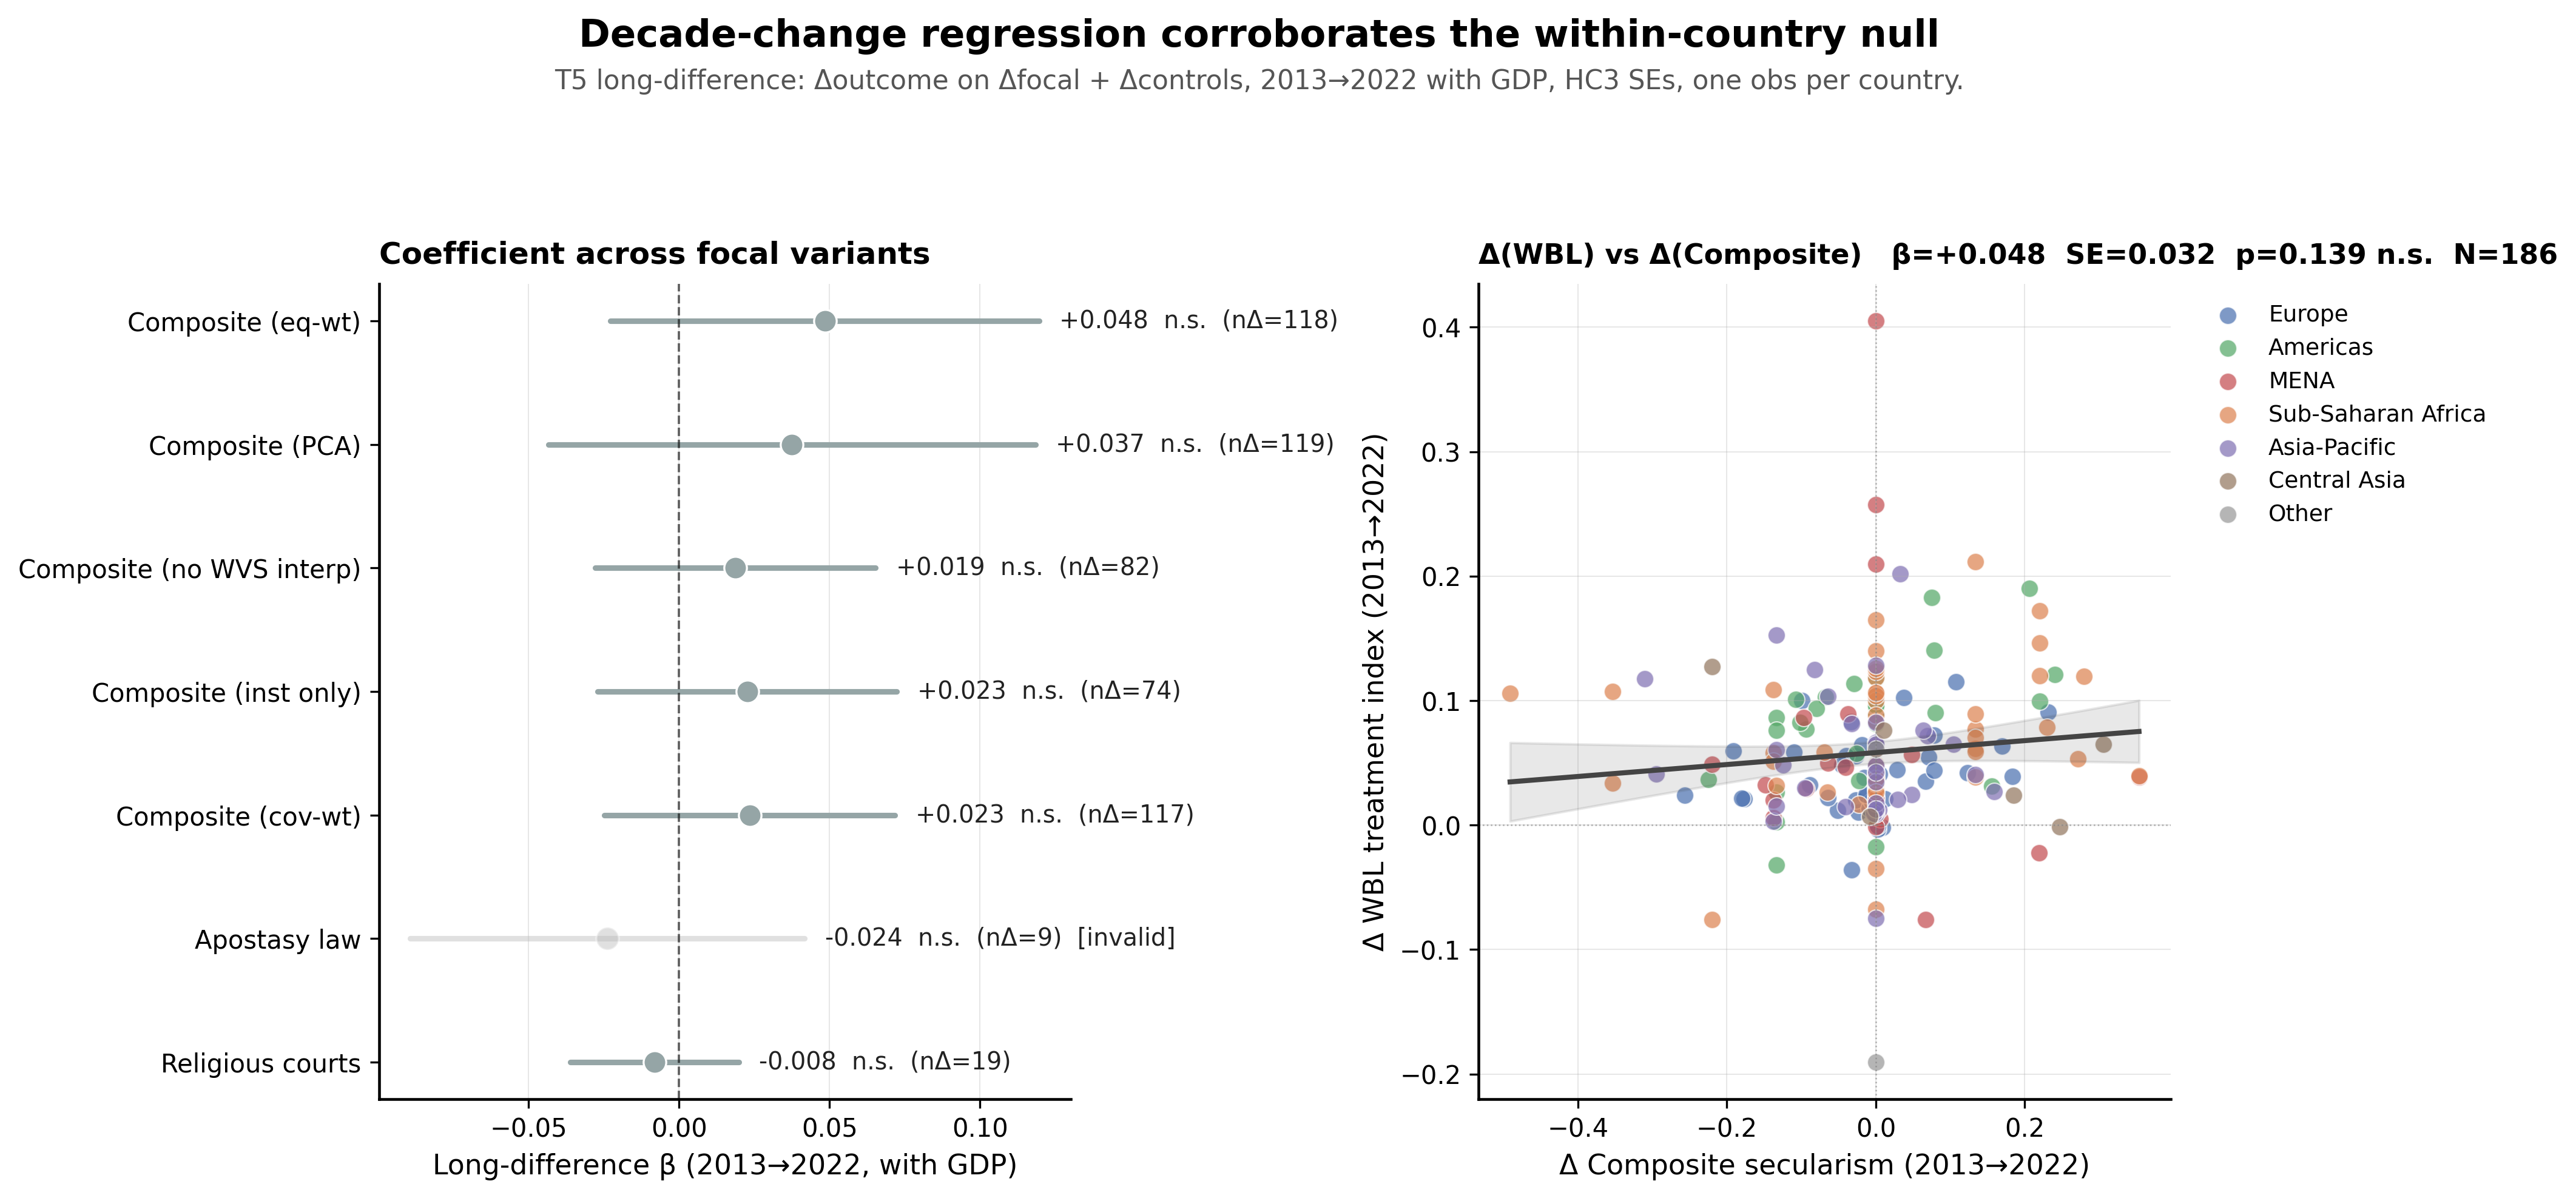
\includegraphics[width=0.95\textwidth]{13_long_difference.png}
\caption{Long-difference regression of the decade-change in the women's treatment index on the decade-change in each focal predictor, 2013--2022 with GDP. Left panel: forest plot of $\hat\beta$ with $95\%$ confidence intervals across seven focal variants. Apostasy is greyed because only nine countries record any apostasy-law movement over the window; courts is flagged low-power with 19 changers. Right panel: decade-change scatter for the headline equal-weight composite, one point per country, region-coloured, with OLS fit and $95\%$ confidence band. Source: \texttt{results/results.csv}, tier \texttt{T5\_long\_diff\_2013\_2022\_with\_gdp}.}
\label{fig:longdiff}
\end{figure}

This appendix reports the two sub-item long-difference results left out of the main Table~\ref{tab:headline} row. Apostasy returns a sign-correct $\hat\beta = -0.042$ ($p = 0.17$) at the 2013--2022 window, identified off only nine changer countries and flagged invalid under our $n_{\text{changers}} \geq 10$ threshold; the sign is consistent with T1/T2/T4 but the estimate is diagnostically fragile. Courts at 19 changer countries falls in the low-power band (10--24) and is reported with that caveat. Alt-endpoint and sub-window variants are in the \texttt{T5\_long\_diff} rows of \texttt{results/results.csv}.

\subsection{WEF Global Gender Gap Caveat}

\begin{figure}[H]
\centering
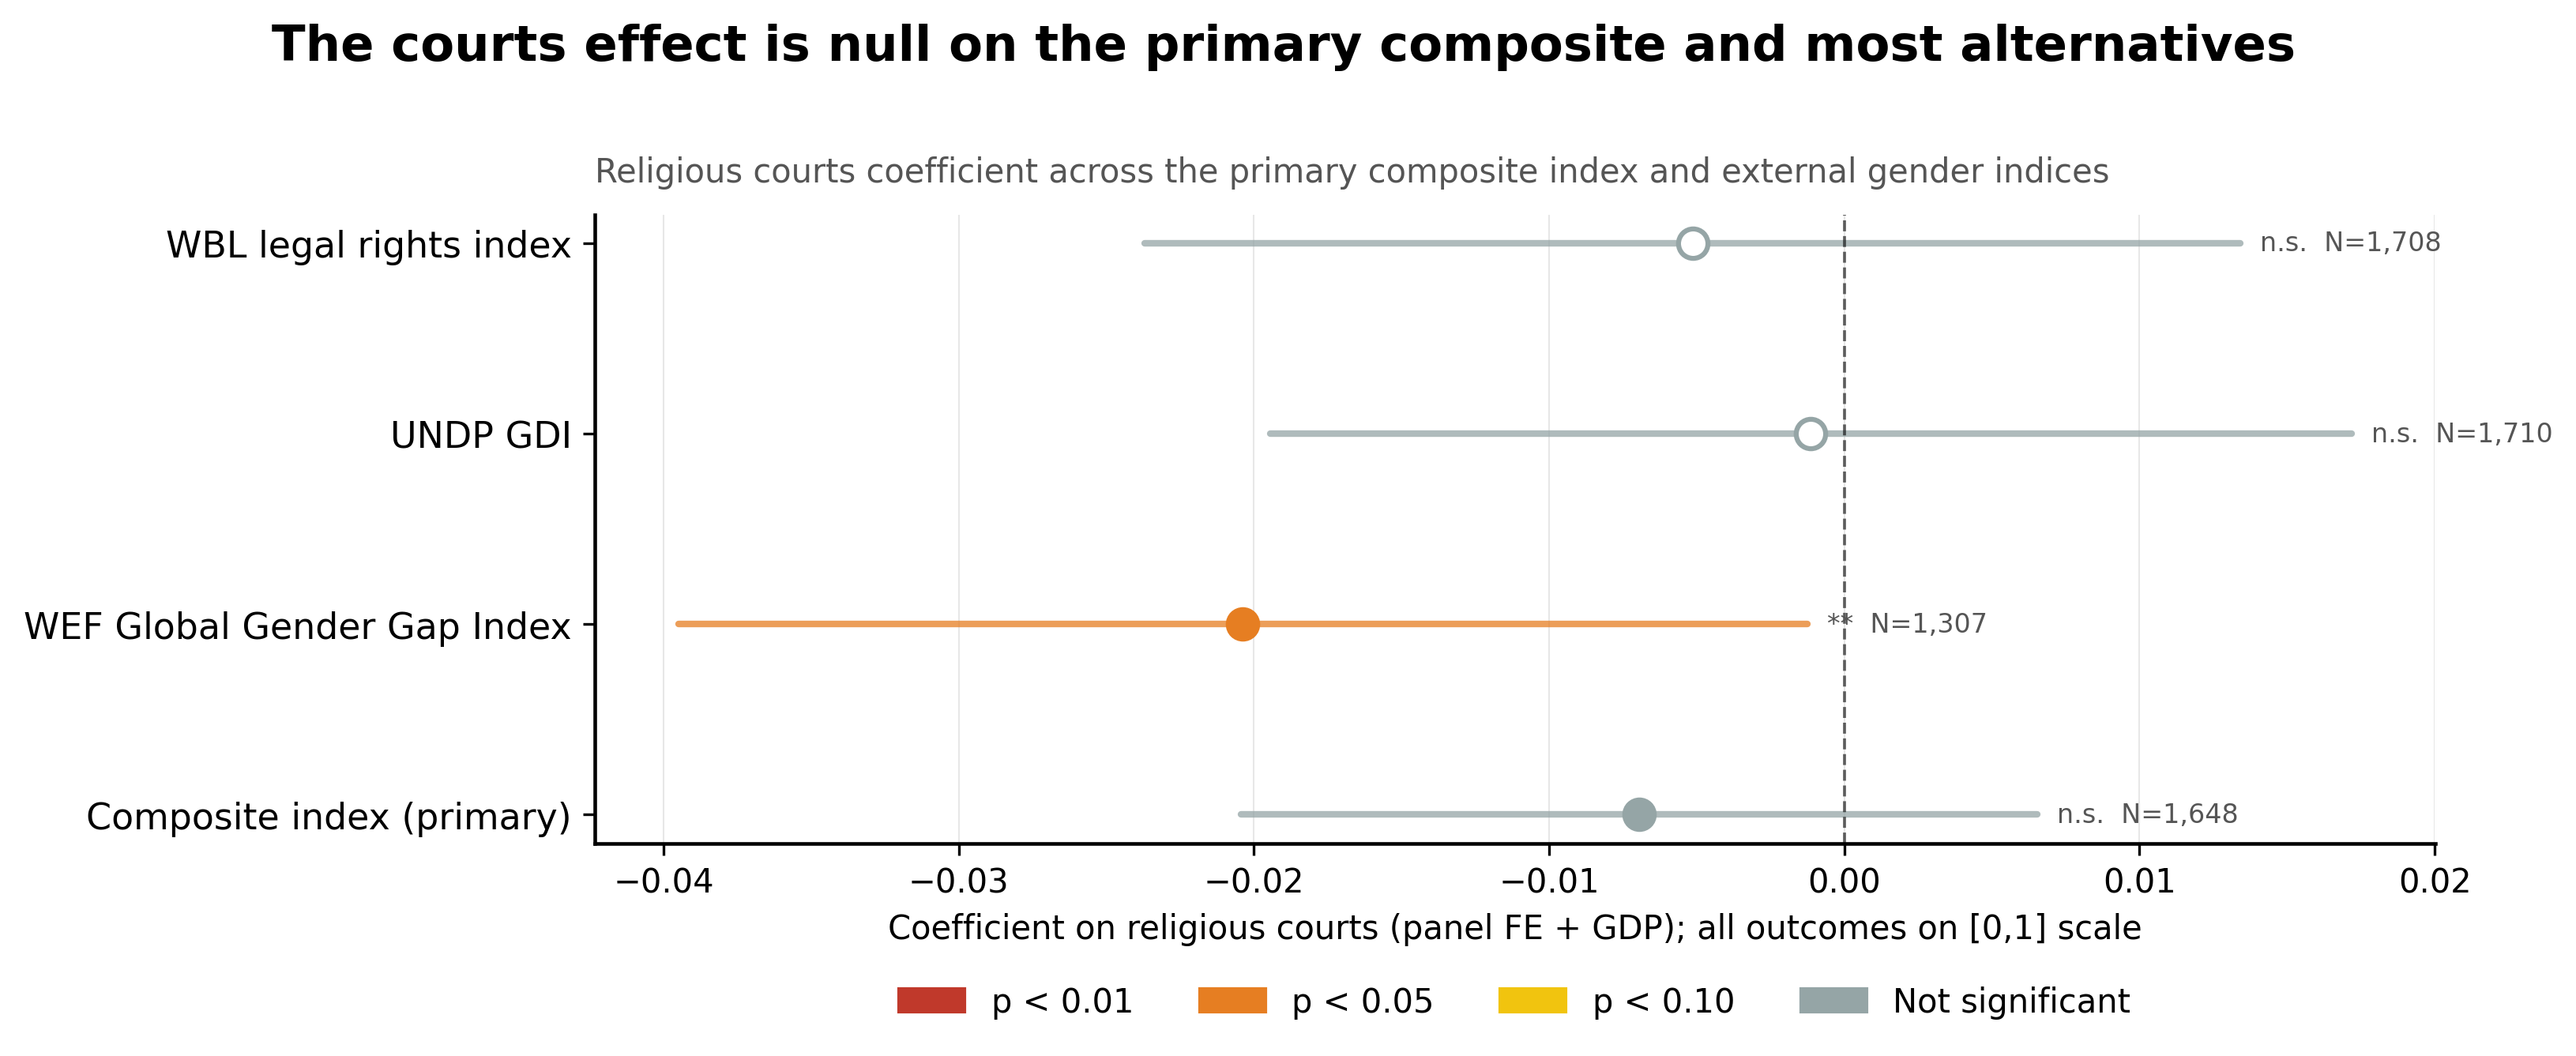
\includegraphics[width=0.85\textwidth]{10_alt_outcomes.png}
\caption{Focal-predictor coefficient (panel FE with GDP) on four alternative outcomes: the primary women's treatment index, the WEF Global Gender Gap, the UNDP Gender Development Index, and the WBL legal rights index. All on $[0, 1]$ scales.}
\label{fig:altout}
\end{figure}

The focal composite within-country coefficient is small and wrong-signed on the primary composite, on the UNDP Gender Development Index, and on the WBL legal rights index, and larger-magnitude negative on the WEF Global Gender Gap. The WEF result pulls in the direction of the cross-sectional prior, which is consistent with the WEF index over-weighting political representation and economic participation in a way that loads on the same structural cross-country clusters that drive the composite's cross-section. We do not adopt the WEF outcome as the headline because the primary composite was pre-specified in \texttt{scoring.py} before the regressions were run; re-running on a different outcome to find a favourable within-country sign would be a garden-of-forking-paths violation. The WEF pattern is disclosed as a caveat rather than a finding.

\subsection{Reverse Causality Test}

The lagged-predictor results (Section 5.5) test the timing of the apostasy effect: contemporaneous and L1 effects are significant; L2 weakens to marginal as the sample shrinks. We additionally tested the reverse direction, regressing future GRI outcomes on the contemporaneous treatment index, and found null effects in both directions. This rules out the most obvious reverse-causality story for the apostasy result.

\subsection{WBL Group Decomposition}

\begin{figure}[H]
\centering
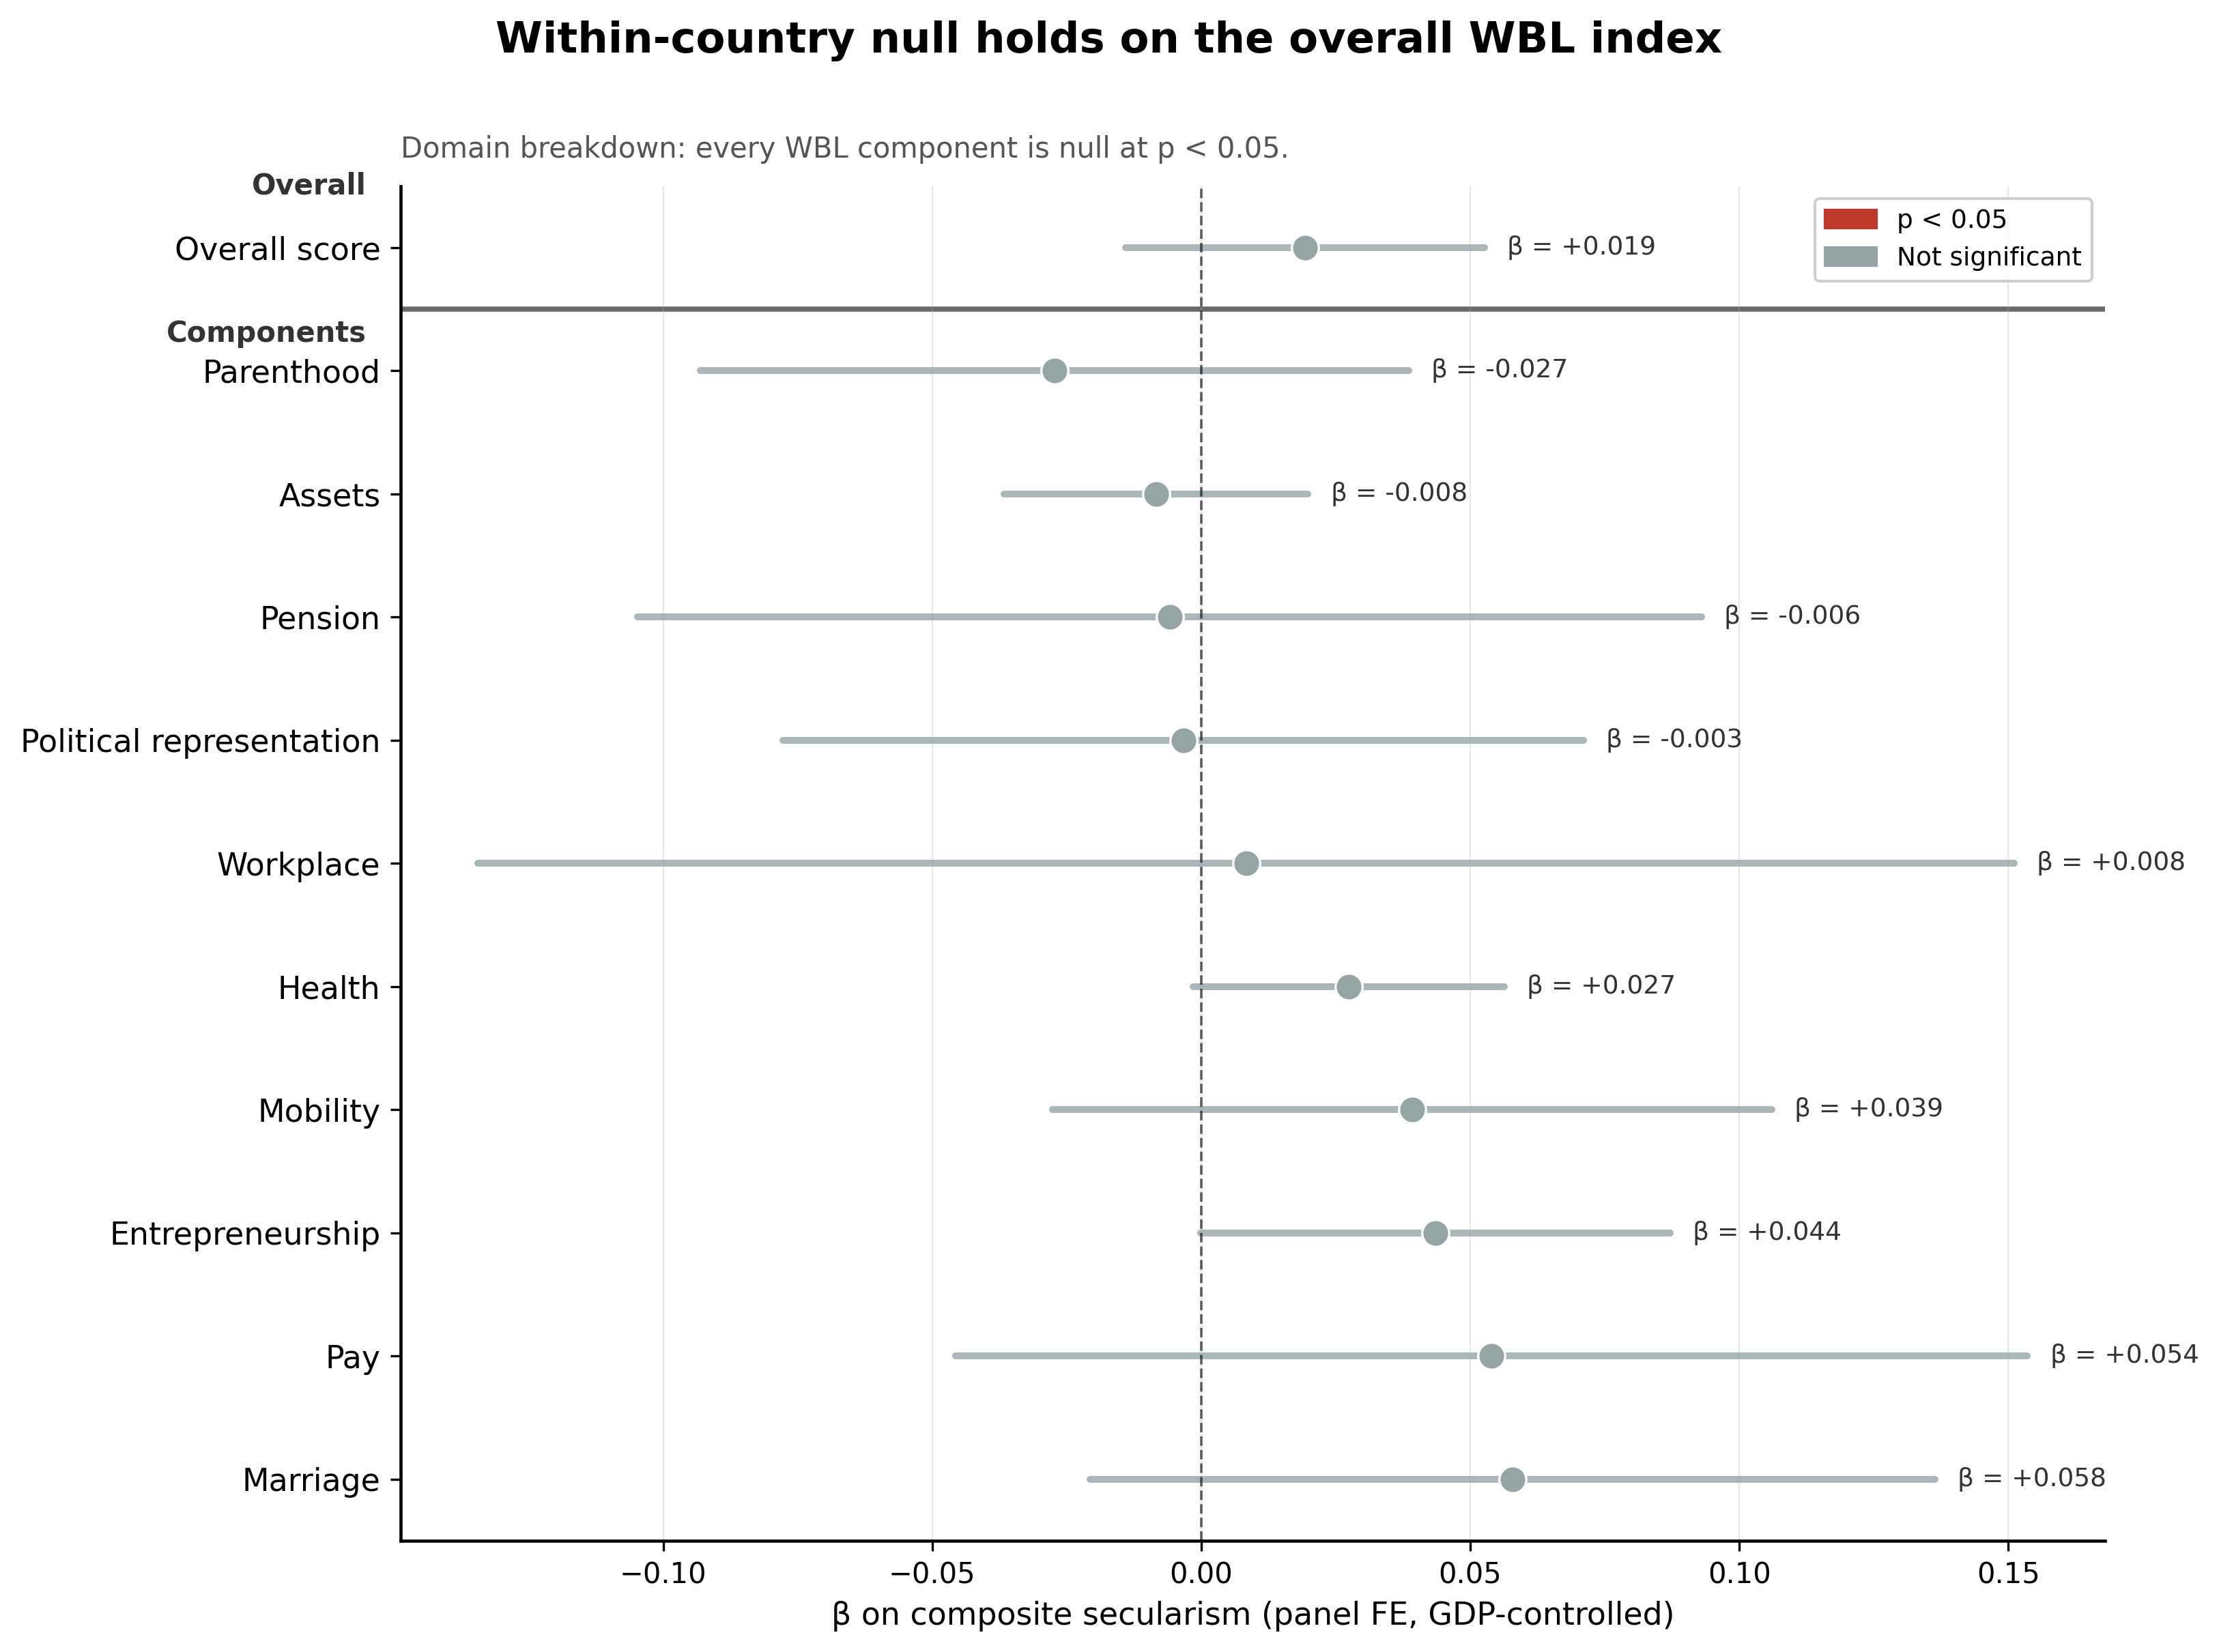
\includegraphics[width=0.85\textwidth]{11_wbl_groups.png}
\caption{Focal-predictor coefficient (panel FE with GDP) across the ten WBL legal-rights subdomains and the overall score.}
\label{fig:wblgroups}
\end{figure}

We checked whether the composite within-country null is an aggregation artefact masking a strong domain-specific effect by re-running the panel FE on each of the ten WBL legal-rights group scores separately. No single domain produces a strong negative within-country composite coefficient. The within-country null is not a composite-outcome artefact; it holds at the most granular level we have.

\subsection{Regional Heterogeneity}

The apostasy effect is strongest in the Sub-Saharan Africa subsample (cross-section coefficient $-0.195$, $p = 0.04$, $n = 47$ in 2013), where apostasy laws cluster in countries with substantial Islamic legal influence. The MENA subsample is too small ($N \approx 18$ in the panel) for meaningful inference but the point estimate is consistent in sign with the global result. The composite's regional pattern mirrors the apostasy pattern: larger negative between-country coefficient in samples that include MENA and Sub-Saharan Africa, weaker elsewhere.

\subsection{Sub-Period Stability}

Restricting the panel to 2013--2019 (excluding the COVID years) produces results numerically similar to the full panel for the composite, for apostasy, and for courts. Pandemic-period composition effects are not driving the headline.

\subsection{Checks Excluded from this Report}

\begin{table}[H]
\centering
\caption{Robustness checks computed but excluded from the body of this report, with the reason for exclusion.}
\label{tab:dropped}
\begin{tabular}{p{0.30\textwidth}p{0.62\textwidth}}
\toprule
Check & Reason for exclusion \\
\midrule
Event studies (all focal predictors) & Designed for sharp policy events; institutional secularism variables move slowly, and the composite's within-country movement is partly interpolator-driven. Pre-trend tests are uninformative by construction at this $T$. \\
Wild cluster bootstrap on the full 166-cluster panel & Redundant with entity-clustered SEs at this cluster count. The wild-cluster bootstrap \emph{is} reported for the T2 changers subsample in \S\ref{sec:wildboot}, where the apostasy focal is identified off only nine changer clusters and the entity-clustered SE is likely too tight. \\
Driscoll--Kraay as a separate headline & Reported in the main table as an SE variant rather than a separate tier. The bandwidth $= 2$ captures within-country autocorrelation over a 10-year window adequately; the DK tightening of the composite and apostasy within-country SEs is included in Table~\ref{tab:headline} for transparency. \\
Mundlak CRE via pooled OLS (Phase 9d) & Identical estimator to T4 with pooled OLS instead of GLS. Same results, no added value. \\
\bottomrule
\end{tabular}
\end{table}

\bibliography{references_full}

\end{document}
